%\documentclass[12pt]{article}

\questionheader{ex:s4.4}


%%%%%%%%%%%%%%%%%%
\subsection*{\Conceptual}
%%%%%%%%%%%%%%%%%%

%%%%%%%%%%%%%%%%%%%%%%%%%%%%%%%
\begin{question}
Each of the figures below contains a sketch of a surface $S$ and
its boundary $\partial S$. Stokes' theorem says that
$\oint_{\partial S}\vF\cdot \dee{\vr}
=\dblInt_S\vnabla\times\vF\cdot\hn\,\dee{S}$
if $\hn$ is a correctly oriented unit normal vector to $S$. 
Add to each sketch a typical such normal vector.
\begin{center}
  (a)\quad \raisebox{-0.9\height}{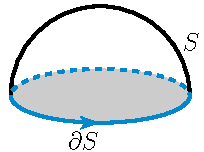
\includegraphics{stokesOrientA.pdf}}\hfil
  (b)\quad \raisebox{-0.9\height}{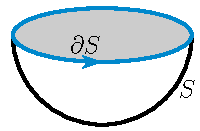
\includegraphics{stokesOrientB.pdf}}\hfil
  (c)\quad \raisebox{-0.9\height}{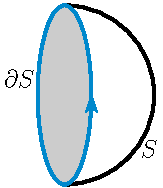
\includegraphics{stokesOrientC.pdf}}
\end{center}
\end{question}

\begin{hint} 
One approach is to first do
\begin{center}
  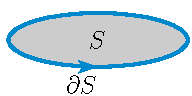
\includegraphics{stokesOrientAh.pdf}
\end{center}
Then imagine slowly deforming the sketch to the get specified $S$'s
\end{hint}

\begin{answer} 
\begin{center}
  (a)\quad \raisebox{-0.9\height}{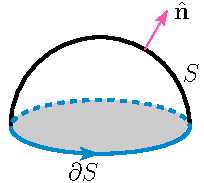
\includegraphics{stokesOrientAs.pdf}}\hfil
  (b)\quad \raisebox{-0.9\height}{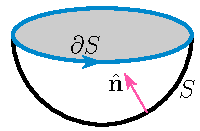
\includegraphics{stokesOrientBs.pdf}}\hfil
  (c)\quad \raisebox{-0.9\height}{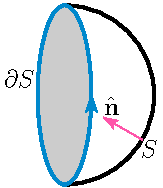
\includegraphics{stokesOrientCs.pdf}}
\end{center}
\end{answer}

\begin{solution} 
One approach is to first consider
\begin{center}
  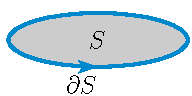
\includegraphics{stokesOrientAh.pdf}
\end{center}
The correct normal to this surface is sketched in 
\begin{center}
  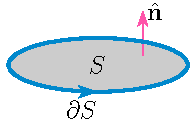
\includegraphics{stokesOrientAhs.pdf}
\end{center}
It is correct because 
    \begin{itemize}\itemsep1pt \parskip0pt \parsep0pt %\itemindent-15pt
    \item
    if you walk along $\partial S$ in the direction of the arrow
    on $\partial S$,
     \item
     with the vector from your feet to your head  having direction $\hn$
    \item
    then $S$ is on your left hand side.
    \end{itemize}
Now pretend that the surface $S$ is made of rubber and that $\hn$ is glued to $S$. We can push on this $S$ to deform it to the $S$ of part (a) or to the $S$
of part (b). This gives the solutions to parts (a) and (b). 
\begin{center}
  (a)\quad \raisebox{-0.9\height}{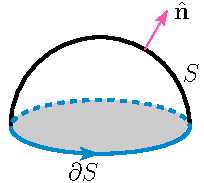
\includegraphics{stokesOrientAs.pdf}}\hfil
  (b)\quad \raisebox{-0.9\height}{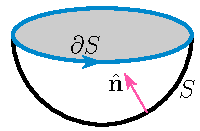
\includegraphics{stokesOrientBs.pdf}}
\end{center}
To deal with part (c), we can first rotate the flat disk that we considered above to get 
\begin{center}
  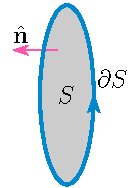
\includegraphics{stokesOrientCh.pdf}
\end{center}
We can push on this $S$ to deform it to the $S$ of part (c). This gives 
the solution to part (c).
\begin{center}
  (c)\quad \raisebox{-0.9\height}{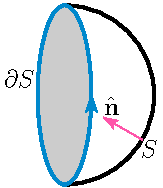
\includegraphics{stokesOrientCs.pdf}}
\end{center}
\end{solution}

%%%%%%%%%%%%%%%%%%%%%%%%%%%%%%%
\begin{question}
Let 
\begin{itemize}\itemsep1pt \parskip0pt \parsep0pt % \itemindent-15pt
\item
$R$ be a finite region in the $xy$-plane,
\item
the boundary, $C$, of $R$ consist of a single piecewise smooth, simple closed curve
    \begin{itemize}\itemsep1pt \parskip0pt \parsep0pt %\itemindent-15pt
     \item
     that is oriented (i.e. an arrow is put on $C$) consistently 
     with $R$ in the sense that if you walk along
     $C$ in the direction of the arrow, then $R$ is on your left
    \end{itemize}
     \begin{center}
        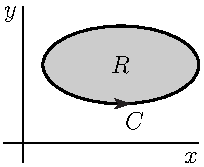
\includegraphics{greens1.pdf}
    \end{center}
\item
$F_1(x,y)$ and $F_2(x,y)$ have continuous first partial derivatives 
at every point of $R$.
\end{itemize}
Use Stokes' theorem to show that
\begin{equation*}
\oint_{C} \big[F_1(x,y)\,\dee{x} +F_2(x,y)\,\dee{y}\big]
 =\dblInt_{R}\Big(\frac{\partial F_2}{\partial x} 
                - \frac{\partial F_1}{\partial y}\Big)\ \dee{x}\dee{y}
\end{equation*}
i.e. to show Green's theorem.

\end{question}

\begin{hint} 
Define the vector field $\vF(x,y,z) = F_1(x,y)\,\hi +F_2(x,y)\,\hj$.
\end{hint}

\begin{answer} 
See the solution.
\end{answer}

\begin{solution} Think of the $xy$-plane as being the plane $z=0$ in $\bbbr^3$.
     \begin{center}
        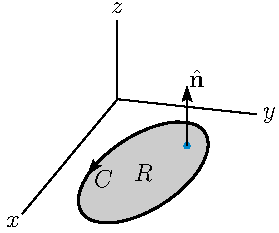
\includegraphics{stokesGreen.pdf}
    \end{center}
We are going to apply Stokes' theorem (Theorem \eref{CLP317}{thm:Stokes} 
in the CLP-4 text) with $S$ being the given region $R$ in the $xy$-plane 
and with $\vF(x,y,z) = F_1(x,y)\,\hi +F_2(x,y)\,\hj$.
Then 
\begin{itemize}\itemsep1pt \parskip0pt \parsep0pt %\itemindent-15p
\item[$\circ$]
the unit normal vector to $S$ specified in Stokes theorem is $\hk$
(if you walk along $\partial S = C$ in the direction of the arrow
    on $C$ with the vector from your feet to your head  having direction $\hk$
    then $S=R$ is on your left hand side) and
\item[$\circ$]
$\dee{S}=\dee{x}\,\dee{y}$ and
\item[$\circ$] the curl of $\vF$ is
\begin{equation*}
\vnabla\times\vF=\det\left[\begin{matrix}\hi & \hj & \hk \\[0.05in]
                  \pdiff{}{x} &
                  \pdiff{}{y} &
                  \pdiff{}{z} \\[0.05in]
                  F_1(x,y) & F_2(x,y) & 0 \end{matrix}\right] 
=\Big(\frac{\partial F_2}{\partial x} 
                - \frac{\partial F_1}{\partial y}\Big)\,\hk
\end{equation*}
\end{itemize}  
So Stokes' theorem gives
\begin{align*}
\oint_{C} \big[F_1(x,y)\,\dee{x} +F_2(x,y)\,\dee{y}\big]
=\oint_{\partial S}\vF\cdot \dee{\vr}
  =\dblInt_{S}\vnabla\times\vF\cdot\hn\ \dee{S}
=\dblInt_{R}\Big(\frac{\partial F_2}{\partial x} 
                - \frac{\partial F_1}{\partial y}\Big)\ \dee{x}\dee{y}
\end{align*}

\end{solution} 

%%%%%%%%%%%%%%%%%%%%%%%%%%%%%%%
\begin{question}
Verify the identity 
$\ \oint_C\phi\vnabla\psi\cdot \dee{\vr}=-\oint_C\psi\vnabla\phi\cdot
                       \dee{\vr}\ $
for any continuously differentiable scalar fields $\phi$ and $\psi$ and
curve $C$ that is the boundary of a piecewise smooth surface.
\end{question}

\begin{hint} 
First verify the vector identity 
$\vnabla\times[\phi\vnabla\psi+\psi\vnabla\phi]=\vZero$
\end{hint}

\begin{answer} 
See the solution.
\end{answer}

\begin{solution} 
We are to show that $\oint_C[\phi\vnabla\psi+\psi\vnabla\phi]\cdot \dee{\vr}=0$.
 Suppose that $C=\partial S$. Then, by Stokes' theorem
\begin{equation*}
\oint_C[\phi\vnabla\psi+\psi\vnabla\phi]\cdot \dee{\vr}
=\dblInt_S\vnabla\times[\phi\vnabla\psi+\psi\vnabla\phi]\cdot\hn\, \dee{S}
\end{equation*}
We will show below %(in two different ways) 
that $\vnabla\times[\phi\vnabla\psi+\psi\vnabla\phi]=\vZero$.
This will imply that $\oint_C[\phi\vnabla\psi+\psi\vnabla\phi]\cdot \dee{\vr}=\vZero$.
One way to see that $\vnabla\times[\phi\vnabla\psi+\psi\vnabla\phi]=\vZero$
is
\begin{align*}
\vnabla\times[\phi\vnabla\psi+\psi\vnabla\phi]
&=\vnabla\times[\vnabla(\phi\psi)] &
&\text{(by part (c) of Theorem \eref{CLP317}{thm:gradIdentities} in the CLP-4 text)}\\
&=\vZero&
&\text{(by part (b) of Theorem \eref{CLP317}{thm:degTwoIdentities} in the CLP-4 text)}
\end{align*}
Another way to see that $\vnabla\times[\phi\vnabla\psi+\psi\vnabla\phi]=\vZero$
is
\begin{align*}
\vnabla\times[\phi\vnabla\psi+\psi\vnabla\phi]
&=\vnabla\phi\times\vnabla\psi+\phi\vnabla\times(\vnabla\psi)
+\vnabla\psi\times\vnabla\phi+\psi\vnabla\times(\vnabla\phi)\\
&=\vnabla\phi\times\vnabla\psi
+\vnabla\psi\times\vnabla\phi\qquad\text{since $\phi\vnabla\times(\vnabla\psi)=\psi\vnabla\times(\vnabla\phi)=\vZero$}\\
&=\vZero
\end{align*}
\end{solution}



%%%%%%%%%%%%%%%%%%
\subsection*{\Procedural}
%%%%%%%%%%%%%%%%%%

%%%%%%%%%%%%%%%%%%%%%%%%%%%
\begin{question}
 Let $C$ be the curve of intersection of the cylinder $x^2+y^2=1$
and the surface $z=y^2$ oriented in the counterclockwise direction as seen
from $(0,0,100)$. Let $\vF=(x^2-y\,,\,y^2+x\,,\,1)$. Calculate 
$\oint_C\vF\cdot \dee{\vr}$
\begin{enumerate}[(a)]
\item by direct evaluation
\item by using Stokes' Theorem.
\end{enumerate}
\end{question}

\begin{hint} 
To parametrize the curve $x^2+y^2=1$, $z=y^2$, first parametrize the 
circle $x^2+y^2=1$. That is, find $x(t)$ and 
$y(t)$ obeying $x(t^2)+y(t)^2=1$. Then set $z(t) =y(t)^2$.
\end{hint}

\begin{answer} 
(a) $2\pi$ \qquad
(b) $2\pi$
\end{answer}

\begin{solution} 
(a) Observe that $x(t)=\cos t$ and $y(t)=\sin t$ obey $x(t)^2+y(t)^2=1$.
Then $z(t)=y(t)^2=\sin ^2 t$.  So we may parametrize the curve by
$\vr(t)=(\cos t, \sin t, \sin^2 t)$ with $0\le t\le 2\pi$.
Then
\begin{align*}
\vr'(t)&=(-\sin t\,,\, \cos t \,,\, 2\sin t\cos t)\\
\vF\big(\vr(t)\big)&=\big(\cos^2t-\sin t\,,\,\sin^2t+\cos t\,,\,1\big)\\
\vF\big(\vr(t)\big)\cdot\vr'(t)&=-\sin t\cos^2 t+\sin^2 t+\sin^2t\cos t
+\cos^2t+2\sin t\cos t\\
&=1+\frac{1}{3}\diff{}{t}[\cos^3t+\sin^3 t]+\sin(2t)\\
\oint_C\vF\cdot \dee{\vr}
&=\int_0^{2\pi}
\left\{1+\frac{1}{3}\diff{}{t}[\cos^3t+\sin^3 t]+\sin(2t)\right\}\,\dee{t} \\
&=\left[t+\frac{1}{3}[\cos^3t+\sin^3 t] -\frac{1}{2}\cos(2t) \right]_0^{2\pi}\\
&=2\pi
\end{align*}

(b) Let $S$ be the surface $z=f(x,y)$ with $f(x,y)=y^2$ 
and $x^2+y^2\le 1$. Since $C$ is oriented counter clockwise when
viewed from high on the $z$-axis, Stokes' theorem requires that we use 
the normal $\hn$ to $S$ with positive $z$ component. Hence
\begin{align*}
\hn\,dS&=\Big[-\pdiff{f}{x}\,\hi
-\pdiff{f}{y}\,\hj+\hk\Big]\,\dee{x}\,\dee{y}
=\Big[-2y\,\hj+\hk\Big]\,\dee{x}\,\dee{y}\\
\vnabla\times\vF&=\det\left[\begin{matrix}\hi & \hj & \hk \\[0.05in]
                  \pdiff{}{x} &
                  \pdiff{}{y} &
                  \pdiff{}{z} \\[0.05in]
                  x^2-y & y^2+x & 1 \end{matrix}\right] 
=2\hk\\
\vnabla\times\vF\cdot\hn\,dS&=2\,\dee{x}\,\dee{y}\\
\oint_C\vF\cdot \dee{\vr}
&=\dblInt_S\vnabla\times\vF\cdot\hn\,\dee{S}
=2\dblInt_{x^2+y^2\le 1}\,\dee{x}\,\dee{y}\\
&=2\pi
\end{align*}

\end{solution}


%%%%%%%%%%%%%%%%%%%%%%%%%%%%%%%
\begin{question}
Evaluate
 $\oint_C \vF\cdot \dee{\vr}$ where $\vF=ye^x\,\hi+(x+e^x)\,\hj+z^2\,\hk$ and
$C$ is the curve 
\begin{equation*}
\vr(t)=(1+\cos t)\,\hi+(1+\sin t)\,\hj+(1-\sin t-\cos t)\,\hk\qquad
0\le t\le 2\pi
\end{equation*}
\end{question}

\begin{hint} 
Apply Stokes' theorem.
Note that $\vr(t) = x(t)\,\hi+y(t)\,\hj +z(t)\,\hk$
obeys $x(t)+y(t)+z(t)=3$, for every $t$, and that $x(t)\,\hi+y(t)\,\hj
=(1+\cos t)\,\hi+(1+\sin t)\,\hj$ runs counterclockwise around
the circle of radius 1 centered on $(1,1)$.
\end{hint}

\begin{answer} 
$\pi$
\end{answer}

\begin{solution} 
We apply Stokes' theorem. First,  
\begin{equation*}
\vnabla\times\vF=\det\left[\begin{matrix}\hi & \hj & \hk \\[0.05in]
                  \pdiff{}{x} &  \pdiff{}{y} & \pdiff{}{z} \\[0.05in]
                  ye^x & x+e^x & z^2 
                 \end{matrix}\right] 
=\big(1+e^x-e^x\big)\,\hk
=\hk
\end{equation*}
Note that $\vr(t) = x(t)\,\hi+y(t)\,\hj +z(t)\,\hk$
obeys $x(t)+y(t)+z(t)=3$, for every $t$, and that $x(t)\,\hi+y(t)\,\hj
=(1+\cos t)\,\hi+(1+\sin t)\,\hj$ runs counterclockwise around
the circle of radius 1 centered on $(1,1)$. So we choose $S$
to be the part of the plane $G(x,y,z)=x+y+z=3$ with $(x-1)^2+(y-1)^2\le 1$.
Then, by Stokes' Theorem,
\begin{equation*}
\oint_C \vF\cdot \dee{\vr}
=\dblInt_S \vnabla\times\vF\cdot \hn\,\dee{S}
=\dblInt_S \hk\cdot \hn\,\dee{S}
\end{equation*}
with
\begin{equation*}
\hn\,\dee{S} = \pm \frac{\vnabla G}{\vnabla G\cdot\hk}\,\dee{x} \dee{y}
= \pm\big(\hi+\hj+\hk\big)\,\dee{x} \dee{y}
\end{equation*}
As $(1+\cos t)\,\hi+(1+\sin t)\,\hj$ runs counterclockwise around
the circle $(x-1)^2+(y-1)^2\le 1$, Stokes' theorem
specifies the plus sign and
\begin{equation*}
\oint_C \vF\cdot \dee{\vr}
=\dblInt_{(x-1)^2+(y-1)^2\le 1} \dee{x}\,\dee{y}
=\pi
\end{equation*}

\end{solution}



%%%%%%%%%%%%%%%%%%%%%%%%%%%%%%%
\begin{question}[M317 2011A] %4
Find the value of
$\dblInt_S\vnabla\times\vF\cdot\hn\,\dee{S}$ where 
$\vF = \big(z - y\,,\, x\,,\, -x\big)$ and $S$ is the hemisphere 
\begin{equation*}
\Set{(x, y, z) \in\bbbr^3 }{ x^2 + y^2 + z^2 = 4,\ z \ge 0} 
\end{equation*}
oriented so the surface normals point away from the centre of the
hemisphere.
\end{question}

\begin{hint} 
The form of the integral should be quite suggestive.
\end{hint}

\begin{answer} 
$8\pi$
\end{answer}

\begin{solution} 
The boundary of $S$ is
\begin{equation*}
\partial S = \Set{(x,y,z)}{z=0,\ x^2+y^2=4}
\end{equation*}
and can be parametrized
\begin{equation*}
\vr(\theta) = 2\cos\theta\,\hi +2\sin\theta\,\hj\qquad
0\le\theta\le 2\pi
\end{equation*}
\begin{center}
     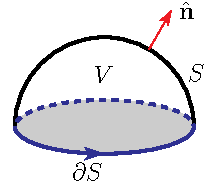
\includegraphics{OE11A_4.pdf}
\end{center}
So, by Stokes' theorem (Theorem \eref{CLP317}{thm:Stokes} in the CLP-4 text)
\begin{align*}
\dblInt_S\vnabla\times\vF\cdot\hn\,\dee{S}
&=\oint_{\partial S}\vF\cdot\dee{\vr} \\
&=\int_0^{2\pi} (\overbrace{-2\sin\theta\,\hi+2\cos\theta\,\hj-2\cos\theta\,\hk}^
               {\vF(\vr(\theta))})\cdot
     (\overbrace{-2\sin\theta\,\hi+2\cos\theta\,\hj}^
                {\vr'(\theta)})\ \dee{\theta} \\
&=4\int_0^{2\pi}\dee{\theta} \\
&=8\pi
\end{align*} 
\end{solution}

%%%%%%%%%%%%%%%%%%%%%%%%%%%
\begin{question}[M317 1998D] %6
 Let $\cS$ be the part of the surface $z=16-{(x^2+y^2)}^2$
which lies above the $xy$-plane. Let $\vF$ be the vector field
$$
\vF=x\ln(1+z)\,\hi+x(3+y)\,\hj+y\cos z\,\hk
$$
Calculate
$$
\dblInt_{\cS}\vnabla\times\vF\cdot\hn\,\dee{S}
$$
where $\hn$ is the upward normal on $\cS$.
\end{question}

\begin{hint} 
The form of the integral should be quite suggestive.
\end{hint}

\begin{answer} 
$12\pi$
\end{answer}


\begin{solution}  \emph{Solution 1}:\ \ \ 
The boundary of $\cS$ is the circle $x^2+y^2=4$, $z=0$.
Let $\cC$ be this circle, oriented by the parametrization $x(t)=2\cos t$, 
$y(t)=2\sin t$, $z(t)=0$. By Stokes' theorem
\begin{align*}
\dblInt_{\cS}\vnabla\times\vF\cdot\hn\,\dee{S}
&=\int_{\cC}\vF\cdot \dee{\vr}
=\int_0^{2\pi}\vF(2\cos t,2\sin t,0)\cdot \diff{\vr}{t}(t)\ \dee{t}\\
&=\int_0^{2\pi}\big[0\,\hi+2\cos t(3+2\sin t)\,\hj+2\sin t\,\hk\big]\cdot 
\big[-2\sin t\,\hi+2\cos t\hj\big]\ \dee{t}\\
&=\int_0^{2\pi}\big[12\cos^2 t+8\cos^2t\sin t\big]\ \dee{t} \\
&=\int_0^{2\pi}\big[6+6\cos(2t)+8\cos^2t\sin t\big]\ \dee{t} \\
&=\Big[6t+3\sin(2t) -\frac{8}{3}\cos^3 t\Big]_0^{2\pi}
=12\pi
\end{align*}
For an efficient, sneaky, way to evaluate 
$\int_0^{2\pi} \cos^2 t\,\dee{t}$, see Example
\eref{CLP317}{eg:workIntegalB} in the CLP-4 text.


\emph{Solution 2}:\ \ \ Let
\begin{itemize}\itemsep1pt \parskip0pt \parsep0pt %\itemindent-15p
\item[$\circ$]
$\cS$ be the surface specified in the question, with upward pointing normal, and
\item[$\circ$]
$\cD$ be the disk $\Set{(x,y,z)}{x^2+y^2\le 4,\ z=0}$, with normal $\hn=\hk$, and
\item[$\circ$]
$\cC$ be the circle $\Set{(x,y,z)}{x^2+y^2=4,\ z=0}$, oriented as in the figure below.
\end{itemize}
\begin{center}
     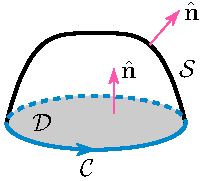
\includegraphics{OE98D_6.pdf}
\end{center}
Note that $\cC$ is the boundary curve for both $\cS$ and $\cD$. So, by
Stokes' theorem, twice 
\begin{align*}
\dblInt_{\cS}\vnabla\times\vF\cdot\hn\,\dee{S}
&=\int_{\cC}\vF\cdot \dee{\vr}
=\dblInt_{\cD}\vnabla\times\vF\cdot\hn\,\dee{S} \\
&=\dblInt_{\cD}\vnabla\times\vF\cdot\hk\,\dee{S}
\end{align*}
Now the $\hk$ component of $\vnabla\times\vF$ is
\begin{align*}
\vnabla\times\vF\cdot\hk
&=\pdiff{}{x}\big[x(3+y)\big]
 - \pdiff{}{y}\big[x\ln(1+z)\big]
=3+y
\end{align*}
%For the given vector field 
%\begin{align*}
%\vnabla\times\vF
%&=\det\left[\begin{matrix}
%\hi &\hj &\hk \\
%\tfrac{\partial\hfill}{\partial x} & \tfrac{\partial\hfill}{\partial y} & 
%                \tfrac{\partial\hfill}{\partial z} \\
%x\ln(1+z) & x(3+y) & y\cos z
%\end{matrix}
%\right] \\
%&=\cos z\,\hi+\tfrac{x}{1+z}\,\hj+(3+y)\hk
%\end{align*}
As $y$ is odd under $y\rightarrow-y$ and $\cD$ is invariant under $y\rightarrow-y$, we have $\dblInt_{\cD}y\,\dee{S}=0$
and
\begin{align*}
\dblInt_{\cS}\vnabla\times\vF\cdot\hn\,\dee{S}
= \dblInt_{\cD}(3+y)\,\dee{S}
=3\dblInt_{\cD}\dee{S}
=3\,\text{Area}(\cS) =3\,\pi 2^2=12\pi
\end{align*}


\end{solution}


%%%%%%%%%%%%%%%%%%%%%%%%%%%
\begin{question}[M317 2001A] %6
Let $\cC$ be the intersection of the paraboloid $z=4-x^2-y^2$
with the cylinder $x^2+(y-1)^2=1$, oriented counterclockwise when viewed
from high on the $z$-axis. Let $\vF=xz\,\hi+x\,\hj+yz\,\hk$. Find
$\oint_{\cC}\vF\cdot \dee{\vr}$. 
\end{question}

\begin{hint} 
What's the title of this section?
\end{hint}

\begin{answer} 
$\pi$
\end{answer}


\begin{solution}
Let $S$ be the portion of the paraboloid $z=f(x,y)=4-x^2-y^2$
with $x^2+(y-1)^2\le 1$ and let $\hn$ be the upward normal to $S$.
For this surface 
$$
\hn\,\dee{S}=\big(-f_x(x,y)\,\hi -f_y(x,y)\,\hj +\hk\big)\dee{x}\dee{y}
   = \big(2x\,\hi+2y\,\hj+\hk\big)\,\dee{x}\dee{y}
$$
by (\eref{CLP317}{eq:SUdSgraph}) in the CLP-4 text. As $(x,y,z)$ runs over
$S$, $(x,y)$ runs over the circular disk
\begin{equation*}
D = \Set{(x,y)}{x^2+(y-1)^2\le 1}
\end{equation*}
For the given vector field 
\begin{align*}
\vnabla\times\vF
&=\det\left[\begin{matrix}
\hi &\hj &\hk \\
\tfrac{\partial\hfill}{\partial x} & \tfrac{\partial\hfill}{\partial y} & 
                \tfrac{\partial\hfill}{\partial z} \\
xz & x & yz
\end{matrix}
\right] \\
&=z\,\hi+x\,\hj+\hk
\end{align*}
so that, by Stokes' theorem  (Theorem \eref{CLP317}{thm:Stokes} in the CLP-4 text),
\begin{align*}
\oint_{\cC}\vF\cdot \dee{\vr}
&=\dblInt_S \vnabla\times\vF\cdot \hn\,\dee{S}\\
&=\dblInt_D
   \big[2x\overbrace{(4-x^2-y^2)}^{z=f(x,y)}+2xy+1\big]\,\dee{x}\dee{y}
\end{align*}
By oddness under $x\rightarrow -x$, all terms integrate to zero except
for the last. So
$$
\oint_{\cC}\vF\cdot \dee{\vr}
=\dblInt_D\,\dee{x}\dee{y}
=\text{Area}(D)
=\pi
$$
\end{solution}


%%%%%%%%%%%%%%%%%%%%%%%%%%%
\begin{question}
Let $\vF = - ye^z\,\hi + x^3\cos z\,\hj + z\sin(xy)\,\hk$, and let 
$S$ be the part of the surface $ z = (1-x^2)(1-y^2)$ that lies above the 
square $-1\le x\le 1$, $-1\le y\le 1$ in the $xy$-plane.  Find 
the flux of $\vnabla\times \vF$ upward through $S$. 
\end{question}

\begin{hint} 
We are to evaluate a flux integral of the form $\dblInt_S\vnabla\times\vF\cdot\hn\,\dee{S}$. Sure looks like
one side of Stokes' theorem.
\end{hint}

\begin{answer} 
$8$
\end{answer}


\begin{solution}
The surface 
\begin{align*}
S&=\Set{(x,y,z)}{-1\le x\le 1,\ -1\le y\le 1,\ z\ge 0,\ z = (1-x^2)(1-y^2)} \\
 &=\Set{(x,y,z)}{-1\le x\le 1,\ -1\le y\le 1,\ \ z = (1-x^2)(1-y^2)}
\end{align*}
Note that when $x=1$ or $x=-1$ or $y=1$ or $y=-1$,
we have $z= (1-x^2)(1-y^2)=0$.  So the boundary of $S$,  call it $C$,
is the boundary of the square $-1\le x,y\le 1$, $z=0$, oriented 
counterclockwise. Here is a sketch of $C$.
\begin{center}
   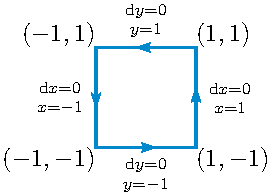
\includegraphics{singGnA.pdf}
\end{center}
Apply Stokes' theorem. Observing that $z=0$ on $C$
so that $\vF = -y\,\hi +x^3\,\hj$,
\begin{align*}
\dblInt_S\vnabla\times\vF\cdot\hn\,\dee{S}
&=\oint_C\vF\cdot \dee{\vr}
=\oint_C[-y\,\hi+x^3\hj]\cdot \dee{\vr}\\
&=\underbrace{\int_{-1}^1 -(-1)\,\dee{x}}_{y=-1{\rm\ side}}
   +\underbrace{\int_{-1}^1 (1)^3\,\dee{y}}_{x=1{\rm\ side}}
   + \underbrace{\int^{-1}_1 -(1)\,\dee{x}}_{y=1{\rm\ side}}
   + \underbrace{\int^{-1}_1 (-1)^3\,\dee{y}}_{x=-1{\rm\ side}} \\
&=8
\end{align*}
\end{solution}


%%%%%%%%%%%%%%%%%%%%%%%%%%%
\begin{question}
Evaluate the integral   $\oint_C \vF\cdot \dee{\vr}$, in which 
$\vF = (e^{x^2} - yz\,,\,\sin y - yz \,,\,xz + 2y)$ and $C$
is the triangular path from $(1, 0, 0)$ to $(0, 1, 0)$ to $(0, 0, 1)$ to 
$(1, 0, 0)$. 
\end{question}

\begin{hint} 
The vector field $\vF$ looks too complicated for a direct evaluation
of the line integral. So, try Stokes' theorem.
\end{hint}

\begin{answer} 
$1$
\end{answer}


\begin{solution}
We shall apply Stokes' Theorem. The curl of $\vF$ is
\begin{equation*}
\vnabla\times\vF=\det\left[\begin{matrix}\hi & \hj & \hk \\[0.05in]
                  \pdiff{}{x} &
                  \pdiff{}{y} &
                  \pdiff{}{z} \\[0.05in]
                  e^{x^2} - yz & \sin y - yz & xz + 2y\end{matrix}\right] 
=(2+y)\,\hi-(z+y)\,\hj+(0+z)\,\hk
\end{equation*}
The curve $C$ is a triangle. All three vertices of the triangle obey
$x+y+z=1$. So the triangle is the boundary
of the surface $S=\Set{(x,y,z)}{x\ge 0,\ y\ge 0,\ z=1-x-y\ge 0}$. 
\begin{center}
   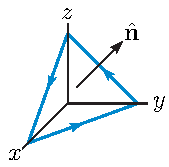
\includegraphics{domainTriangleA.pdf}
\end{center}
The equation of the surface is $z=f(x,y)=1-x-y$.
So, by (\eref{CLP317}{eq:SUdSgraph}) in the CLP-4 text, 
\begin{align*}
\hn\ \dee{S}
&=\big(-f_x\,\hi-f_y\,\hj+\hk\big)\,\dee{x}\,\dee{y}\\
&=(\hi+\hj+\hk)\,\dee{x}\,\dee{y}
\end{align*}
Here $\hn$ is the upward pointing unit normal.
The set of points $(x,y)$ for which there is a corresponding $(x,y,z)$
in $S$ is  $T=\Set{(x,y)}{x\ge 0,\ y\ge 0,\ x+y\le 1}$, which is a triangle
of area $\frac{1}{2}$.
Since $\vnabla\times\vF\cdot\hn\,\dee{S}
=[(2+y)\hi-(z+y)\hj+(0+z)\hk]\cdot(\hi+\hj+\hk)\,\dee{x}\,\dee{y}
= 2\,\dee{x}\,\dee{y}$,
\begin{align*}
%\smash{\figplace{domainTriangleA}{-0.5in}{-1.0in}\hskip.5in}
\oint_C\vF\cdot \dee{\vr}&=\dblInt_S\vnabla\times\vF\cdot\hn\,\dee{S}\\
&=\dblInt_T 2\ \dee{x}\,\dee{y}
= 2\,\text{Area}(T)
=1
\end{align*}
\end{solution}



%%%%%%%%%%%%%%%%%%%%%%%%%%%%%%%
\begin{question}[M317 2001D] %4
Let $\vF(x,y,z)=-z\,\hi+x\,\hj+y\,\hk$ be a vector field. Use
Stokes' theorem to evaluate the line integral 
$
\oint_C\vF\cdot \dee{\vr}
$
where $C$ is the intersection of the plane $z=y$ and the ellipsoid 
$\frac{x^2}{4}+\frac{y^2}{2}+\frac{z^2}{2}=1$, oriented 
counter-clockwise when viewed from high on the  $z$-axis.

\end{question}

%\begin{hint} 
%
%\end{hint}

\begin{answer} 
$4\pi$
\end{answer}

\begin{solution}
Stokes' theorem, which is Theorem \eref{CLP317}{thm:Stokes}
in the CLP-4 text, says that $\oint_C\vF\cdot \dee{\vr}
=\dblInt_S\nabla\times\vF\cdot\hn\,\dee{S}$ for any surface $S$ whose boundary is
$C$. For the given vector field
\begin{align*}
\nabla\times\vF(x,y,z)
&=\det\left[\begin{matrix}
\hi &\hj &\hk \\
\tfrac{\partial\hfill}{\partial x} & \tfrac{\partial\hfill}{\partial y} & 
                \tfrac{\partial\hfill}{\partial z} \\
-z & x & y
\end{matrix}
\right] \\
&=\hi-\hj+\hk
\end{align*}
Choose 
\begin{align*}
S &= \Set{(x,y,z)}{z=y,\ \tfrac{x^2}{4}+\tfrac{y^2}{2}+\tfrac{z^2}{2}\le 1} \\
  &= \Set{(x,y,z)}{z=y,\ \tfrac{x^2}{4}+y^2\le 1}
\end{align*}
to be the part of the plane $z=y$ bounded by the ellipsoid.

\begin{center}
   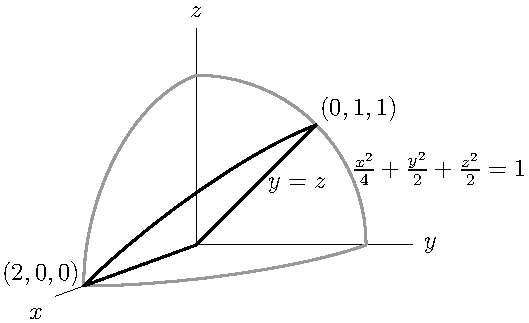
\includegraphics{OE01DQ4.pdf}
\end{center}

As $S$ is part of the plane $z=f(x,y)=y$, (\eref{CLP317}{eq:SUdSgraph})
of the CLP-4 text, gives that
\begin{align*}
\hn\,\dee{S} &=\pm \big(-f_x\,,\,-f_y\,,\, 1\big)\dee{x}\dee{y} \\
&=\pm (0\,,\,-1\,,\, 1)\dee{x}\dee{y} 
\end{align*}
As $C$ has the standard orientation (counter-clockwise when viewed 
from high on the $z$-axis), we want $\hn$ to have a positive $z$-component. 
So 
$\hn\,\dee{S}= (0\,,\,-1\,,\, 1)\dee{x}\dee{y} $.
From the second form of $S$ given above, we see that as $(x,y,z)$
runs over $S$, $(x,y)$ runs over
\begin{equation*}
D=\Set{(x,y)}{\tfrac{x^2}{4}+y^2\le 1}
\end{equation*}
Consequently, Stokes' theorem gives that
\begin{align*}
\oint_C\vF\cdot \dee{\vr}
%&=\dblInt_S\nabla\times\vF\cdot\hn\,\dee{S} \\
&=\dblInt_D\overbrace{(1,-1,1)}^{\nabla\times\vF}\cdot
            \overbrace{(0\,,\,-1\,,\, 1)\dee{x}\dee{y} }^{\hn\,\dee{S}} \\
&=2\dblInt_D \dee{x}\dee{y}
=2\,\text{Area}(D)
\end{align*}
The ellipse $D$, that is $\tfrac{x^2}{4}+y^2\le 1$, has semi-axes
$a=2$ and $b=1$ and hence area $\pi ab=2\pi$. Finally
\begin{equation*}
\oint_C\vF\cdot \dee{\vr}
=2\,\text{Area}(D)
=4\pi
\end{equation*}
\end{solution}


%%%%%%%%%%%%%%%%%%%%%%%%%%%%%%%
\begin{question}[M317 2016D] %9
Consider the vector field $\vF(x,y, z) = z^2 \,\hi + x^2 \,\hj + y^2\,\hk$ 
in $\bbbr^3$.
\begin{enumerate}[(a)]
\item
Compute the line integral $I_1 = \int_{C_1}\vF\cdot\dee{\vr}$
where $C_1$ is the curve consisting of three line segments, 
$L_1$ from $(2, 0, 0)$ to $(0, 2, 0)$, then 
$L_2$ from $(0, 2, 0)$ to $(0, 0, 2)$, finally 
$L_3$ from $(0, 0, 2)$ to $(2, 0, 0)$.
\item
A simple closed curve $C_2$ lies on the plane $E\,:\, x + y + z = 2$, 
enclosing a region $R$ on the plane of area $3$, and oriented in a 
counterclockwise direction as observed from the positive $x$-axis. 
Compute the line integral $I_2 = \int_{C_2}\vF\cdot\dee{\vr}$.

\end{enumerate}
\end{question}

%\begin{hint} 
%
%\end{hint}

\begin{answer} 
(a) $8$\qquad
(b) $4\sqrt{3}$
\end{answer}

\begin{solution} 
Note that the curve of part (a) is a simple closed curve
that lies in the plane $x+y+z=2$ and is oriented in a 
counterclockwise direction as observed from the positive $x$-axis.
The curve of part (a) encloses a triangle. 
\vadjust{
\begin{center}
     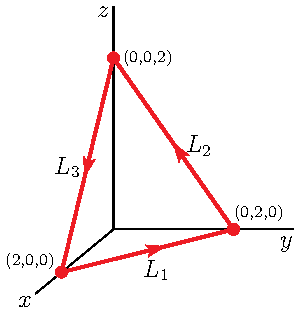
\includegraphics{OE16D_9.pdf}
\end{center}
}
Two of the sides of the triangle
are $(0,2,0)-(2,0,0)=(-2,2,0)$ and  $(0,0,2)-(0,2,0)=(0,-2,2)$ so the
area of the triangle is
\begin{equation*}
\frac{1}{2}\big|(-2,2,0)\times (0,-2,2)\big|
=\frac{1}{2} \det\left[\begin{matrix}\hi&\hj&\hk\\[0.03in] 
     -2& 2& 0 \\  0 & -2 & 2 \end{matrix}\right]
=\frac{1}{2}\big|(4,4,4)\big|
=2\sqrt{3}
\end{equation*}
So let's do part (b) first.

(b) We are not told explicitly what $C_2$ is, so we certainly can't
do a direct evaluation. Instead, let's use Stokes' theorem
(Theorem \eref{CLP317}{thm:Stokes} in the CLP-4 text). The curl of $\vF$ is
\begin{align*}
\vnabla\times\vF
&=\det\left[\begin{matrix}
\hi &\hj &\hk \\
\tfrac{\partial\hfill}{\partial x} & \tfrac{\partial\hfill}{\partial y} & 
                \tfrac{\partial\hfill}{\partial z} \\
z^2 & x^2 & y^2
\end{matrix}
\right] \\
&= 2y\,\hi 
    +2z\,\hj 
    +2x\,\hk  
\end{align*}
The upward pointing unit normal to $E$ is $\hn=\frac{\hi+\hj+\hk}{\sqrt{3}}$.
So, by Stokes' theorem,
\begin{align*}
I_2 &= \int_{C_2}\vF\cdot\dee{\vr}
    =\dblInt_R \vnabla\times\vF\cdot\hn\,\dee{S}
    =\dblInt_R \big(2y\,\hi +2z\,\hj +2x\,\hk\big)\cdot
               \frac{\hi+\hj+\hk}{\sqrt{3}}\,\dee{S} \\
&=\frac{2}{\sqrt{3}}\dblInt_R \big(\overbrace{y + z + x}^
                             {=2\ {\rm on}\ R}\big)\,\dee{S}
%=\frac{2}{\sqrt{3}}\dblInt_R 2\,\dee{S}
=\frac{4}{\sqrt{3}}\text{Area}(R)
=4\sqrt{3}
\end{align*}

(a) Denote by $T$ the triangle enclosed by $C_1$. By the
computation that we have just done in part (b) 
\begin{align*}
I_1 &= \int_{C_1}\vF\cdot\dee{\vr}
     =\frac{4}{\sqrt{3}}\text{Area}(T)
     =8
\end{align*}
\end{solution}

%%%%%%%%%%%%%%%%%%%%%%%%%%%
\begin{question}[M317 2017A] %5
Let $C = C_1 + C_2 + C_3$ be the curve given by the union of the 
three parameterized curves
\begin{alignat*}{3}
\vr_1(t) &= \big(2\cos t, 2\sin t, 0\big), &\qquad
&0 \le t \le \pi/2 \\
\vr_2(t) &= \big(0, 2\cos t, 2\sin t\big), &
&0 \le t \le \pi/2 \\
\vr_3(t) &= \big(2\sin t, 0, 2\cos t\big), &
&0 \le t \le \pi/2
\end{alignat*}
\begin{enumerate}[(a)]
\item
Draw a picture of $C$. Clearly mark each of the curves $C_1$, $C_2$, and $C_3$
and indicate the orientations given by the parameterizations.


\item
Find and parameterize an oriented surface $S$ whose boundary is $C$ 
(with the given orientations).

\item
Compute the line integral $\int_C \vF\cdot\dee{\vr}$ where
\begin{equation*}
\vF = \Big(y + \sin(x^2)\,,\, z - 3x + \ln(1 + y^2)\,,\, y + e^{z^2}\Big)
\end{equation*}

\end{enumerate}
\end{question}

%\begin{hint} 
%\end{hint}

\begin{answer} 
(a)
\begin{center}
     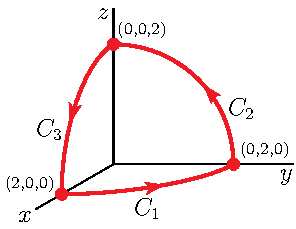
\includegraphics{OE17A_5}
\end{center}

(b) $S=\Set{(x,y,z)}{x^2+y^2+z^2=4,\ x\ge 0,\ y\ge 0,\ z\ge 0}$
with 
\begin{equation*}
\vr(\theta,\varphi)
= 2\cos\theta\sin\varphi\ \hi
+ 2\sin\theta\sin\varphi\ \hj
+ 2\cos\varphi\ \hk,\qquad
0\le\theta\le\frac{\pi}{2},\ 
0\le\varphi\le\frac{\pi}{2}
\end{equation*}
and
\begin{equation*}
\hn = \cos\theta\sin\varphi\ \hi
            +\sin\theta\sin\varphi\ \hj
            +\cos\varphi\ \hk
=\frac{1}{2}\,\vr(\theta,\varphi)
\end{equation*}

(c) $-4\pi$
\end{answer}

\begin{solution} 
(a) Observe that
\begin{itemize}\itemsep1pt \parskip0pt \parsep0pt %\itemindent-15p
\item[$\circ$]
the curve $C_1$ is one quarter of a circle in the $xy$-plane,
centred on the origin, of radius $2$, starting at $(2,0,0)$ and
ending at $(0,2,0)$ and
\item[$\circ$]
the curve $C_2$ is one quarter of a circle in the $yz$-plane,
centred on the origin, of radius $2$, starting at $(0,2,0)$ and
ending at $(0,0,2)$ and
\item[$\circ$]
the curve $C_3$ is one quarter of a circle in the $xz$-plane,
centred on the origin, of radius $2$, starting at $(0,0,2)$ and
ending at $(2,0,0)$.
\end{itemize}     
Here is a sketch.
\begin{center}
     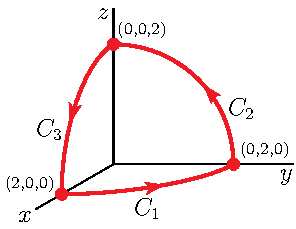
\includegraphics{OE17A_5}
\end{center}

(b) $C$ lies completely on the sphere $x^2+y^2+z^2=4$. So it is natural
to choose
\begin{equation*}
S=\Set{(x,y,z)}{x^2+y^2+z^2=4,\ x\ge 0,\ y\ge 0,\ z\ge 0}
\end{equation*}
and to parametrize $S$ using spherical coordinates
\begin{equation*}
\vr(\theta,\varphi)
= 2\cos\theta\sin\varphi\ \hi
+ 2\sin\theta\sin\varphi\ \hj
+ 2\cos\varphi\ \hk,\qquad
0\le\theta\le\frac{\pi}{2},\ 
0\le\varphi\le\frac{\pi}{2}
\end{equation*}
Since
\begin{align*}
\frac{\partial\vr}{\partial\theta}
&= -2\sin\theta\sin\varphi\,\hi +2\cos\theta\sin\varphi\,\hj  \\
\frac{\partial\vr}{\partial\varphi}
&= 2\cos\theta\cos\varphi\,\hi +2\sin\theta\cos\varphi\,\hj 
  - 2\sin\varphi\,\hk
\end{align*}
so that
\begin{align*}
\frac{\partial\vr}{\partial\theta}\times\frac{\partial\vr}{\partial\varphi}
&= \det\left[\begin{matrix} \hi & \hj & \hk \\[0.05in]
-2\sin\theta\sin\varphi & 2\cos\theta\sin\varphi & 0 \\[0.05in]
2\cos\theta\cos\varphi & 2\sin\theta\cos\varphi & - 2\sin\varphi
         \end{matrix}\right] \\
&= -4\cos\theta\sin^2\varphi\ \hi
   -4\sin\theta\sin^2\varphi\ \hj
   -4\sin\varphi\cos\varphi\ \hk
\end{align*}
(\eref{CLP317}{eq:SUdSparam}) in the CLP-4 text gives
\begin{align*}
\hn\,\dee{S} = \pm \frac{\partial\vr}{\partial\theta}\times
            \frac{\partial\vr}{\partial\varphi}\,\dee{\theta}\dee{\varphi}
= \mp 4\big(\cos\theta\sin\varphi\ \hi
            +\sin\theta\sin\varphi\ \hj
            +\cos\varphi\ \hk\big)
          \sin\varphi\ \dee{\theta}\dee{\varphi}
\end{align*}
We want $\hn$ to point outward, for compatibility with the orientation
of $C$. So we choose the $+$ sign.
\begin{align*}
\hn\,\dee{S} 
= 4\big(\cos\theta\sin\varphi\ \hi
            +\sin\theta\sin\varphi\ \hj
            +\cos\varphi\ \hk\big)
          \sin\varphi\ \dee{\theta}\dee{\varphi}
=2\,\vr(\theta,\varphi)\sin\varphi\ \dee{\theta}\dee{\varphi}
\end{align*}

(c) The vector field $\vF$ looks too complicated for a direct evaluation
of the line integral. So, in preparation for an application of Stokes'
theorem, we compute
\begin{align*}
\vnabla\times\vF&=\det\left[\begin{matrix}\hi&\hj&\hk\\[0.03in] 
     \frac{\partial\hfill}{\partial x}&
        \frac{\partial\hfill}{\partial y}&
        \frac{\partial\hfill}{\partial z}\\[0.03in]
 y + \sin(x^2) & z - 3x + \ln(1 + y^2) & y + e^{z^2}\end{matrix}\right] \\
&= -4\,\hk
\end{align*}
So, by Stokes' theorem (Theorem \eref{CLP317}{thm:Stokes} in the CLP-4 text), 
\begin{align*}
\int_C\vF\cdot\dee{\vr}
&=\dblInt_S\vnabla\times\vF\cdot\hn\,\dee{S} \\
&= \int_0^{\pi/2}\dee{\varphi}\int_0^{\pi/2}\dee{\theta}\ 
\big(-4\hk\big)\cdot
\big(\cos\theta\sin\varphi\ \hi
            +\sin\theta\sin\varphi\ \hj
            +\cos\varphi\ \hk\big)\ 
          4\sin\varphi \\
&=-16 \int_0^{\pi/2}\dee{\varphi}\int_0^{\pi/2}\dee{\theta}\ 
              \cos\varphi\sin\varphi 
=16\ \frac{\pi}{2}\ \frac{\cos^2\varphi}{2}\bigg|_0^{\pi/2}\\
&=-4\pi
\end{align*}
\end{solution}


%%%%%%%%%%%%%%%%%%%%%%%%%%%
\begin{question}[M317 2016A] %4
We consider the cone with equation $z = \sqrt{x^2 + y^2}$. Note that its tip, 
or vertex, is located at the origin $(0, 0, 0)$. The cone is oriented 
in such a way that the normal vectors point downwards (and away from 
the $z$ axis). In the parts below, both $S_1$ and $S_2$ are 
oriented this way.

Let $\vF = \big(-zy, zx, xy \cos(yz)\big)$.

\begin{enumerate}[(a)]
\item
Let $S_1$ be the part of the cone that lies between the planes 
$z = 0$ and $z = 4$. Note that $S_1$ does not include any part of 
the plane $z = 4$. Use Stokes' theorem to determine the value of
\begin{equation*}
\dblInt_{S_1} \vnabla\times\vF \cdot \hn\,\dee{S}
\end{equation*}
Make a sketch indicating the orientations of $S_1$ and of the 
contour(s) of integration.

\item
Let $S_2$ be the part of the cone that lies below the plane 
$z = 4$ and above $z = 1$. Note that $S_2$ does not include any part 
of the planes $z = 1$ and $z = 4$. Determine the flux of $\vnabla\times\vF$ across $S_2$. Justify your answer, including a sketch indicating the
orientations of $S_2$ and of the contour(s) of integration.
\end{enumerate}
\end{question}

%\begin{hint} 
%\end{hint}

\begin{answer} 
(a) $-128\pi$,\qquad
(b) $-126\pi$
\end{answer}


\begin{solution}
 (a)
The boundary, $\partial S_1$, of $S_1$ as specified in Stokes' theorem (Theorem
\eref{CLP317}{thm:Stokes} in the CLP-4 text) is the circle
$\sqrt{x^2+y^2}=4$, $z=4$ oriented \emph{clockwise} when viewed from high on
the $z$-axis. That is, we can parametrize $\partial S_1$ by
\begin{align*}
\vr(t) = 4\cos t\,\hi -4\sin t\,\hj +4\,\hk,\qquad 0\le t\le 2\pi
\end{align*} 
So
\begin{align*}
\vF\big(\vr(t)\big)\cdot\dee{\vr}
&= \big(16\sin t \,,\, 16\cos t \,,\, -16\sin t\cos t \cos(-16\sin t)  \big)
      \cdot
   \big(-4\sin t \,,\, -4\cos t \,,\, 0\big)\,\dee{t} \\
&= -64\,\dee{t}
\end{align*}
and, by Stokes' theorem,
\begin{align*}
\dblInt_{S_1} \vnabla\times\vF \cdot \hn\,\dee{S}
&= \oint_{\partial S_1} \vF\big(\vr(t)\big)\cdot\dee{\vr}
= -64 \int_0^{2\pi} \dee{t}
=-128\pi
\end{align*}

\begin{center}
       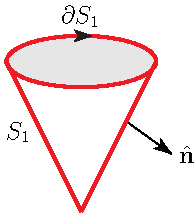
\includegraphics{conePa.pdf}\qquad\qquad
       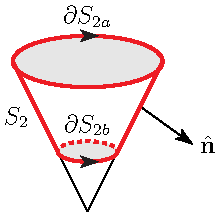
\includegraphics{conePb.pdf}
\end{center}


\noindent (b)
The boundary, $\partial S_2$, of $S_2$ consists of two parts,
a circle in the plane $z=4$ and a circle in the plane $z=1$.
We'll call the first part $\partial S_{2a}$. It is the same as
$\partial S_1$. We'll call the second part $\partial S_{2b}$.
It is the circle $\sqrt{x^2+y^2}=1$, $z=1$ oriented \emph{counterclockwise} 
when viewed from high on the $z$-axis. 
We can parametrize it
\begin{align*}
\vr(t) = \cos t\,\hi +\sin t\,\hj + \hk,\qquad 0\le t\le 2\pi
\end{align*} 
So, on $\partial S_{2b}$,
\begin{align*}
\vF\big(\vr(t)\big)\cdot\dee{\vr}
&= \big(-\sin t \,,\, \cos t \,,\, \sin t\cos t \cos(\sin t)  \big)
      \cdot
   \big(-\sin t \,,\, \cos t \,,\, 0\big)\,\dee{t} \\
&= \dee{t}
\end{align*}
and, by Stokes' theorem,
\begin{align*}
\dblInt_{S_2} \vnabla\times\vF \cdot \hn\,\dee{S}
&= \oint_{\partial S_{2a}} \vF\big(\vr(t)\big)\cdot\dee{\vr}
   +\oint_{\partial S_{2b}} \vF\big(\vr(t)\big)\cdot\dee{\vr}
= -128\pi +  \int_0^{2\pi} \dee{t} \\
&=-126\pi
\end{align*}
\end{solution}

%%%%%%%%%%%%%%%%%%%%%%%%%%%
\begin{question}[M317 2015A] %5
Consider the curve $C$ that is the intersection of the plane $z = x + 4$ 
and the cylinder $x^2 + y^2 = 4$, and suppose $C$ is oriented so that 
it is traversed \emph{clockwise} as seen from above.

Let $\vF(x, y, z) = \big(x^3 + 2y\,,\, \sin(y) + z\,,\, x + \sin(z^2)\big)$.

Use Stokes' Theorem to evaluate the line integral
$\oint_C\vF\cdot\dee{\vr}$. 
\end{question}

%\begin{hint} 
%\end{hint}

\begin{answer} 
$4\pi$
\end{answer}


\begin{solution}
Denote by
\begin{equation*}
S=\Set{(x,y,z)}{z=x+4,\ x^2+y^2\le 4}
\end{equation*}
the part of the plane $z=x+4$ that is contained in the cylinder
$x^2+y^2=4$. Orient $S$ by the downward pointing normal 
$\hn =\frac{1}{\sqrt{2}}(1,0,-1)$. Then $C$ is the boundary of $S$.
The part of $C$ and $S$ that are in the first octant are sketched below.
 \begin{center}
    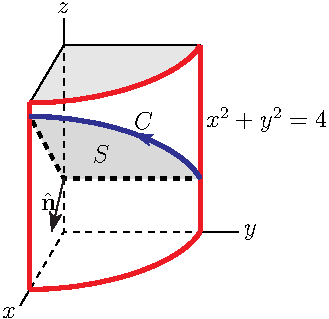
\includegraphics{OE15A_5.pdf}
\end{center}
We may parametrize $S$ by
\begin{equation*}
\vr(x,y) = (x,y, x+4)\qquad\text{with}\quad x^2+y^2\le 4
\end{equation*}
So,
\begin{equation*}
\frac{\partial\vr}{\partial x}\times\frac{\partial\vr}{\partial y}
= \det\left[\begin{matrix} \hi & \hj & \hk \\
1 & 0 & 1 \\
0 & 1 & 0 \end{matrix}\right]
= \big(-1, 0, 1\big)
\end{equation*}
and, by (\eref{CLP317}{eq:SUdSparam}) in the CLP-4 text,
\begin{align*}
\hn\,\dee{S} = -\frac{\partial\vr}{\partial x}\times
            \frac{\partial\vr}{\partial y}\,\dee{x}\dee{y}
= (1,0,-1)\,\dee{x}\dee{y}
\end{align*}
We have chosen to ``$-$'' sign in $\hn\,\dee{S} = 
       \pm\frac{\partial\vr}{\partial x}\times
        \frac{\partial\vr}{\partial y}\,\dee{x}\dee{y}$
to give the downward pointing normal. As the curl of $\vF$ is
\begin{align*}
\vnabla\times\vF
&=\det\left[\begin{matrix}
\hi &\hj &\hk \\
\tfrac{\partial\hfill}{\partial x} & \tfrac{\partial\hfill}{\partial y} & 
                \tfrac{\partial\hfill}{\partial z} \\
x^3 + 2y & \sin(y) + z &  x + \sin(z^2)
\end{matrix}
\right] \\
&= -\hi -\hj -2\hk
\end{align*}
Stokes' theorem (Theorem \eref{CLP317}{thm:Stokes} in the CLP-4 text) gives
\begin{align*}
\oint_C\vF\cdot\dee{\vr}
&=\dblInt_S\vnabla\times\vF\cdot\hn\,\dee{S} 
=\dblInt_S (-1,-1,-2)\cdot(1,0,-1)\,\dee{x}\dee{y} 
=\dblInt_S \dee{x}\dee{y} 
=4\pi
\end{align*}
\end{solution}

%%%%%%%%%%%%%%%%%%%%%%%%%%%
\begin{question}
\begin{enumerate}[(a)]
\item
Consider the vector field $\vF(x, y, z) = (x+y^2\,,\, 2y+4z^2\,,\,3z+2x^2)$ in 
$\bbbr^3$. Compute the line integral $\oint_C \vF\cdot\dee{\vr}$, where 
$C$ is the curve consisting of the three line segments,
$L_1$ from $(2, 0, 0)$ to $(0, 2, 0)$, then 
$L_2$ from $(0, 2, 0)$ to $(0, 0, 1)$, and finally 
$L_3$ from $(0, 0, 1)$ to $(2, 0, 0)$.
\item
A simple closed curve $C$ lies in the plane $x + y + 2z = 2$. 
The surface this curve $C$ surrounds inside the plane $x + y + 2z = 2$ 
has area $6$. The curve $C$ is oriented in a counterclockwise
direction as observed from the positive x-axis.
Compute the line integral $\oint_C\vF\cdot \dee{\vr}$ , where $\vF$ 
is as in (a).
\end{enumerate}
\end{question}

\begin{hint} 
All three vertices of part (a) lie in the plane of part (b).
\end{hint}

\begin{answer} 
(a) -8\qquad
(b) $-8\sqrt{6}$
\end{answer}


\begin{solution}
(a) Note that all three vertices, $(2,0,0)$, $(0,2,0)$ and $0,0,1)$, lie in the
plane $x+y+2z=2$. So the entire path lies in that plane too. 
\vadjust{
\begin{center}
       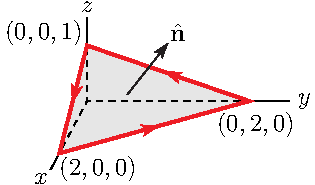
\includegraphics{OE13DB_4.pdf}
\end{center}
}
In part (b)
we will need to evaluate a line integral that clearly cannot be computed
directly --- we will need to use Stokes' theorem. So let's use
Stokes' theorem in part (a) too. First, we find
\begin{align*}
\vnabla\times\vF
&=\det\left[\begin{matrix}
\hi &\hj &\hk \\
\tfrac{\partial\hfill}{\partial x} & \tfrac{\partial\hfill}{\partial y} & 
                \tfrac{\partial\hfill}{\partial z} \\
x+y^2 & 2y+4z^2 & 3z+2x^2
\end{matrix}
\right]
=-8z\,\hi - 4x\,\hj - 2y\,\hk
\end{align*}
Let $S$ be the triangular surface that is contained in the plane 
$x+y+2z=2$ and is bounded by $L_1$, $L_2$ and $L_3$. Orient $S$ by the normal vector $\hn = \frac{1}{\sqrt{6}}(\hi+\hj+2\hk)$. Then, 
\begin{equation*}
\vnabla\times\vF\cdot\hn
=\frac{1}{\sqrt{6}}\big(-8z\,\hi - 4x\,\hj - 2y\,\hk\big)\cdot(\hi+\hj+2\hk)
=-\frac{4}{\sqrt{6}}(x+y+2z)
\end{equation*}
and, by Stokes' theorem,
\begin{align*}
\oint_C\vF\cdot \dee{\vr}
&=\dblInt_S\vnabla\times\vF\cdot\hn\,\dee{S}
=-\frac{4}{\sqrt{6}}\dblInt_S(x+y+2z)\,\dee{S}
=-\frac{8}{\sqrt{6}}\dblInt_S\dee{S}
=-\frac{8}{\sqrt{6}}\text{Area}(S)
\end{align*}
The triangle $S$ is half of the parallelogram with sides $(0,2,0)-(2,0,0)
=(-2,2,0)$ and $(0,0,1)-(2,0,0)=(-2,0,1)$. The area of the parallelogram
is
\begin{align*}
\big|(-2,2,0)\times (-2,0,1)\big|
=\big|(2,2,4)\big|
=2\sqrt{6}
\end{align*}
So
\begin{align*}
\oint_C\vF\cdot \dee{\vr} = -\frac{8}{\sqrt{6}} \sqrt{6}
=-8
\end{align*}

\noindent (b)
Let $\tilde S$ be the specified surface. Then, as in part (a), 
\begin{align*}
\oint_C\vF\cdot \dee{\vr}
&=\dblInt_{\tilde S}\vnabla\times\vF\cdot\hn\,\dee{S}
=-\frac{4}{\sqrt{6}}\dblInt_{\tilde S}(x+y+2z)\,\dee{S}
=-\frac{8}{\sqrt{6}}\dblInt_{\tilde S}\dee{S}
=-\frac{8}{\sqrt{6}}\text{Area}(\tilde S) \\
&=-8\sqrt{6}
\end{align*}
\end{solution}

%%%%%%%%%%%%%%%%%%%%%%%%%%%
\begin{question}[M317 2009A] %7
Evaluate the line integral
\begin{equation*}
\int_C\left(z+\frac{1}{1+z}\right)\dee{x}
         +xz\,\dee{y}
         +\left(3xy-\frac{x}{(z+1)^2}\right)\dee{z}
\end{equation*}
where $C$ is the curve parameterized by
\begin{equation*}
\vr(t) = \big(\cos t\,,\, \sin t\,,\, 1 - \cos^2 t \sin t\big)\qquad
0 \le t \le 2\pi
\end{equation*}
\end{question}

\begin{hint} 
The curve $C$ is the boundary of a surface. To guess the surface
express the $z$ component of $\vr(t)$ in terms of the $x$ and $y$ components.
\end{hint}

\begin{answer} 
$5\pi/4$
\end{answer}


\begin{solution}
 Let's try Stokes' theorem with
\begin{equation*}
\vF = \left(z+\frac{1}{1+z}\right)\hi
         +xz\,\hj
         +\left(3xy-\frac{x}{(z+1)^2}\right)\hk
\end{equation*}
The curl of $\vF$ is
\begin{align*}
\vnabla\times\vF
&=\det\left[\begin{matrix}
\hi &\hj &\hk \\
\tfrac{\partial\hfill}{\partial x} & \tfrac{\partial\hfill}{\partial y} & 
                \tfrac{\partial\hfill}{\partial z} \\
z+\frac{1}{1+z} & xz & 3xy-\frac{x}{(z+1)^2}
\end{matrix}
\right] \\
&=(3x-x)\hi
  -\left(3y-\frac{1}{(z+1)^2}-1+\frac{1}{(1+z)^2}\right)\hj +z\,\hk \\
&=2x\,\hi +(1-3y)\,\hj+z\,\hk
\end{align*}
Write
\begin{equation*}
S=\Set{(x,y,z)}{z=f(x,y)=1-x^2y,\ x^2+y^2\le 1}
\end{equation*}
For $S$, with the upward pointing normal, by (\eref{CLP317}{eq:SUdSgraph})
of the CLP-4 text,
\begin{align*}
\hn\,\dee{S} &=\big(-f_x\,,\,-f_y\,,\, 1\big)\dee{x}\dee{y} \\
&=\big(2xy\,,\,x^2\,,\, 1\big)\dee{x}\dee{y} 
\end{align*}
so that
\begin{align*}
\vnabla\times\vF\cdot\hn\,\dee{S}
&=\big\{4x^2y + (x^2-3x^2y) +\overbrace{(1-x^2y)}^{z}\big\}\,\dee{x}\dee{y}
\end{align*}
and, by Stokes' theorem,
\begin{align*}
\int_C \vF\cdot\dee{\vr}
=\dblInt_S \vnabla\times\vF\cdot\hn\,\dee{S}
=\dblInt_{x^2+y^2\le 1}
  \big\{4x^2y + x^2-3x^2y + 1-x^2y\big\}\,\dee{x}\dee{y}
\end{align*}
So
\begin{align*}
\int_C \vF\cdot\dee{\vr}
&=\dblInt_{x^2+y^2\le 1}
  \big\{x^2+ 1\big\}\,\dee{x}\dee{y}
=\pi + \dblInt_{x^2+y^2\le 1} x^2\,\dee{x}\dee{y}
\end{align*}
To evaluate the final remaining integral, let's switch to polar coordinates.
\begin{align*}
\dblInt_{x^2+y^2\le 1} x^2\,\dee{x}\dee{y}
&=\int_0^1\dee{r}\ r\int_0^{2\pi}\dee{\theta}\  \big(r\cos\theta)^2 \\
&=\int_0^1 \dee{r}\ r^3\int_0^{2\pi}\dee{\theta}\ \cos^2\theta
\end{align*}
Since \begin{align*}
\int_0^{2\pi}\cos^2\theta\ \dee{\theta}
&=\int_0^{2\pi}\frac{1+\cos(2\theta)}{2}\ \dee{\theta}
=\left[\frac{\theta}{2}+\frac{\sin(2\theta)}{4}\right]_0^{2\pi}
=\pi
\end{align*}
we finally have
$\int_0^1 \dee{r}\ r^3\int_0^{2\pi}\dee{\theta}\ \cos^2\theta=\frac{\pi}{4}$
and
\begin{equation*}
\int_C \vF\cdot\dee{\vr}
=\pi+\frac{\pi}{4}
=\frac{5\pi}{4}
\end{equation*}
For an efficient, sneaky, way to evaluate 
$\int_0^{2\pi} \cos^2\theta\,\dee{\theta}$,
see Example \eref{CLP317}{eg:workIntegalB} in the CLP-4 text.
\end{solution}

%%%%%%%%%%%%%%%%%%%%%%%%%%%
\begin{question}[M317 2008D] %9
A simple closed curve $C$ lies in the plane $x + y + z = 1$. 
The surface this curve $C$ surrounds inside the plane $x + y + z = 1$
has area $5$. The curve $C$ is oriented in a clockwise direction as 
observed from the positive $z$-axis looking down at the plane
$x + y + z = 1$.

Compute the line integral of $\vF (x, y, z) = (z^2 , x^2 , y^2)$ around $C$.
\end{question}

\begin{hint} 
The fact that the surface is not completely specified is a big hint.
\end{hint}

\begin{answer} 
$-\frac{10}{\sqrt{3}}$
\end{answer}


\begin{solution}
We are to evaluate a line integral around a curve $C$. We are told that 
$C$ is the boundary of a surface $S$ that is contained in the plane 
$x+y+z=1$, but we are not told precisely what $C$ is. So we are going to have to use Stokes' theorem. The curl of $\vF$ is
\begin{align*}
\vnabla\times\vF
&=\det\left[\begin{matrix}
\hi &\hj &\hk \\
\tfrac{\partial\hfill}{\partial x} & \tfrac{\partial\hfill}{\partial y} & 
                \tfrac{\partial\hfill}{\partial z} \\[0.05in]
z^2 & x^2 & y^2
\end{matrix}
\right]
= 2y\,\hi + 2z\,\hj +2x\,\hk
\end{align*}
and, by (\eref{CLP317}{eq:SUdSimplicit}) of the CLP-4 text with 
$G(x,y,z)=x+y+z$, 
\begin{align*}
\dee{S} &= \left|\frac{\vnabla\vG}{\vnabla\vG\cdot\hk}\right|\dee{x}\dee{y}
        =\sqrt{3}\,\dee{x}\dee{y} \\
\hn\,\dee{S} &= \pm \frac{\vnabla\vG}{\vnabla\vG\cdot\hk}\dee{x}\dee{y}
= \pm \big(\hi+\hj+\hk)\,\dee{x}\dee{y}
= \pm \frac{1}{\sqrt{3}} \big(\hi+\hj+\hk)\,\dee{S}
\end{align*}
Because $C$ is oriented in a clockwise direction as 
\vadjust{
\begin{center}
       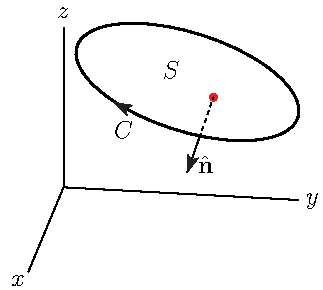
\includegraphics{stokes8.pdf}
\end{center}
}
observed from the positive $z$-axis looking down at the plane, 
$\hn$ is to point downwards, so that
\begin{equation*}
\hn\,\dee{S} = -\frac{1}{\sqrt{3}} \big(\hi+\hj+\hk)\,\dee{S}
\end{equation*}
On $S$ we have $x+y+z=1$, so that Stokes' theorem gives
\begin{align*}
\oint_C\vF\cdot\dee{\vr}
&=\dblInt_S (\vnabla\times\vF)\cdot\hn\,\dee{S}
=\dblInt_S 2(y\,\hi+z\,\hj+x\,\hk)\cdot
        \left(-\frac{1}{\sqrt{3}}\right) \big(\hi+\hj+\hk)\,\dee{S} \\
&=-\frac{2}{\sqrt{3}}\dblInt_S (y+z+x)\,\dee{S}
=-\frac{2}{\sqrt{3}}\dblInt_S \dee{S}
=-\frac{10}{\sqrt{3}}
\end{align*}
since $S$ has area $5$.
\end{solution}

%%%%%%%%%%%%%%%%%%%%%%%%%%%
\begin{question}[M317 2008A] %8
Let $C$ be the oriented curve consisting of the 5 line segments which 
form the paths from $(0, 0, 0)$ to $(0, 1, 1)$, 
               from $(0, 1, 1)$ to $(0, 1, 2)$, 
               from $(0, 1, 2)$ to $(0, 2, 0)$, 
               from $(0, 2, 0)$ to $(2, 2, 0)$,
           and from $(2, 2, 0)$ to $(0, 0, 0)$. 
Let
\begin{equation*}
\vF = (-y+e^x\sin x)\,\hi
         +y^4\,\hj
         +\sqrt{z}\tan z\,\hk
\end{equation*}
Evaluate the integral $\int_C\vF\cdot\dee{\vr}$.
\end{question}

\begin{hint} 
We are to evaluate the line integral of a complicated vector field
around a relatively complicated closed curve. (Sketch it!)
That certainly suggests that
we should not try to evaluate the integral directly.
\end{hint}

\begin{answer} 
$-2$
\end{answer}


\begin{solution}
We are to evaluate the line integral of a complicated vector field
around a relatively complicated closed curve. 
That certainly suggests that
we should not try to evaluate the integral directly. To see if
Stokes' theorem looks promising, let's compute the curl
\begin{align*}
\vnabla\times\vF
&=\det\left[\begin{matrix}
\hi &\hj &\hk \\
\tfrac{\partial\hfill}{\partial x} & \tfrac{\partial\hfill}{\partial y} & 
                \tfrac{\partial\hfill}{\partial z} \\[0.05in]
-y+e^x\sin x & y^4 & \sqrt{z}\tan z
\end{matrix}
\right]
=\hk
\end{align*}
That's suggestive. Next we need to find a surface whose boundary is $C$.
First, here is a sketch of $C$.
\vadjust{
\begin{center}
       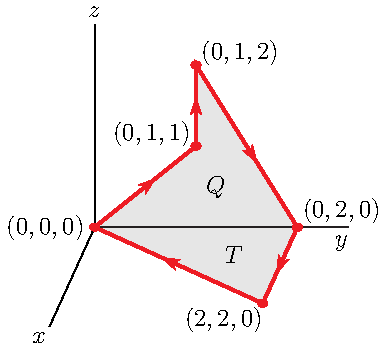
\includegraphics{OE08A_8.pdf}
\end{center}
}
We can choose the surface $S$ to be the union of two flat parts:
\begin{itemize}\itemsep1pt \parskip0pt \parsep0pt %\itemindent-15pt
\item[$\circ$]
the quadralateral $Q$ in the $yz$-plane with vertices $(0,0,0)$,
$(0,1,1)$, $(0,1,2)$ and $(0,2,0)$ and
\item[$\circ$]
the triangle $T$ in the $xy$-plane with vertices $(0,0,0)$,
$(0,2,0)$ and $(2,2,0)$.
\end{itemize} 
The normal to $Q$ is $-\hi$ and the normal to $T$ is $-\hk$. Then Stokes'
theorem gives
\begin{align*}
\int_C\vF\cdot\dee{\vr}
&=\dblInt_S  \vnabla\times\vF\cdot\hn\,\dee{S} \\
&=\dblInt_Q  \hk\cdot(-\hi)\,\dee{S} + \dblInt_T  \hk\cdot(-\hk)\,\dee{S} \\
&= - \dblInt_T \dee{S} \\
&=-\text{Area}(T) \\
&= -\half\overbrace{2}^{\text{base}}\overbrace{2}^{\text{height}} \\
&=-2
\end{align*}
\end{solution}

%%%%%%%%%%%%%%%%%%%%%%%%%%%
\begin{question}[M317 2007A] %8
Suppose the curve $C$ is the intersection of the cylinder 
$x^2 + y^2 = 1$ with the surface $z = xy^2$, traversed clockwise if 
viewed from the positive z-axis, i.e. viewed ``from above''. 
Evaluate the line integral
\begin{equation*}
\int_C  (z + \sin z) \,\dee{x} 
      + (x^3 - x^2 y) \,\dee{y} 
      + (x \cos z - y) \,\dee{z}
\end{equation*}
\end{question}

\begin{hint} 
The integral looks messy. Compute the curl of
$\vF$ to help gauge if Stokes' theorem would be easier.
\end{hint}

\begin{answer} 
$-\pi$
\end{answer}


\begin{solution}
The integral looks messy. Let's compute the curl of
\begin{equation*}
\vF = (z + \sin z) \,\hi 
      + (x^3 - x^2 y) \,\hj
      + (x \cos z - y) \,\hk
\end{equation*} 
to help gauge if Stokes' theorem would be easier.
\begin{align*}
\vnabla\times\vF
&=\det\left[\begin{matrix}
\hi &\hj &\hk \\
\tfrac{\partial\hfill}{\partial x} & \tfrac{\partial\hfill}{\partial y} & 
                \tfrac{\partial\hfill}{\partial z} \\
z + \sin z & x^3 - x^2 y & x \cos z - y
\end{matrix}
\right]
=-\hi +\hj +(3x^2-2xy)\,\hk
\end{align*}
That's a lot simpler than $\vF$.
For the surface $z=f(x,y)=xy^2$, with downward pointing normal (since $C$ is traversed clockwise)
\begin{equation*}
\hn\,\dee{S} = -\big(-f_x,-f_y,1\big)\,\dee{x}\dee{y}
=\big(y^2,2xy,-1\big)\,\dee{x}\dee{y}
\end{equation*}
by (\eref{CLP317}{eq:SUdSgraph}) of the CLP-4 text,
So, writing
\begin{align*}
   S&=\Set{(x,y,z)}{z=xy^2,\ x^2+y^2\le 1} \\
   D&=\Set{(x,y)}{x^2+y^2\le 1}
\end{align*} 
Stoke's theorem gives
\begin{align*}
\int_C\vF\cdot\dee{\vr}
&=\dblInt_S \vnabla\times\vF\cdot\hn\,\dee{S}
=\dblInt_D\big\{-y^2+2xy -3x^2+2xy\big\}\,\dee{x}\dee{y} \\
&=-\dblInt_{x^2+y^2\le 1}\big\{3x^2+y^2-4xy\big\}\,\dee{x}\dee{y}
\end{align*}
To evaluate this integral, switch to polar coordinates.
\begin{align*}
\int_C\vF\cdot\dee{\vr}
&=-\int_0^1\dee{r}\ r\int_0^{2\pi}\dee{\theta}\ 
           \big\{3r^2\cos^2\theta+r^2\sin^2\theta
              -4r^2\sin\theta\cos\theta\big\} \\
&=-4\pi \int_0^1\dee{r}\ r^3 =-\pi
\end{align*}
since 
$\int_0^{2\pi}\sin\theta\cos\theta\,\dee{\theta}
 =\frac{1}{2}\int_0^{2\pi}\sin(2\theta)\,\dee{\theta}=0$
and
$\int_0^{2\pi}\sin^2\theta\,\dee{\theta}
        =\int_0^{2\pi}\cos^2\theta\,\dee{\theta}
        =\pi$.
(See Example \eref{CLP317}{eg:workIntegalB} in the CLP-4 text.)
\end{solution}

%%%%%%%%%%%%%%%%%%%%%%%%%%%
\begin{question}[M317 2006A] %6
Evaluate $\dblInt_S \vnabla\times\vF\cdot\hn\,\dee{S}$ where $S$ is that part 
of the sphere $x^2+y^2+z^2=2$ above the plane $z=1$, $\hn$ is the upward
unit normal, and
\begin{align*}
\vF(x,y,z) = -y^2\,\hi  +x^3\,\hj + \big(e^x + e^y +z\big)\,\hk 
\end{align*}

\end{question}

\begin{hint} 
The form of the integrand is sugestive.
\end{hint}

\begin{answer} 
$\frac{3\pi}{4}$
\end{answer}


\begin{solution}
Here is a sketch of the part of $S$ in the first octant.

\begin{center}
       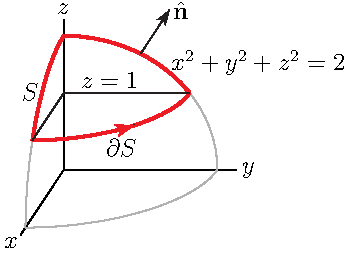
\includegraphics{OE06A_6.pdf}
\end{center}

The boundary, $\partial S$, of $S$ is the circle $x^2+y^2=1$, $z=1$, oriented counterclockwise when viewed from above. 
It is parametrized by
\begin{equation*}
\vr(\theta) = \cos\theta\,\hi + \sin\theta\,\hj + \hk
\qquad 0\le \theta\le 2\pi
\end{equation*}
So Stokes' theorem gives
\begin{align*}
\dblInt_S \vnabla\times\vF\cdot\hn\,\dee{S}
  & = \oint_{\partial S}\vF\cdot\dee{\vr} \\
  & = \int_0^{2\pi} \Big(\overbrace{
        -\sin^2\theta\,\hi +\cos^3\theta\,\hj+(\text{mess})\hk
               }^{\vF(\vr(t))}\Big)\cdot
   \big(\overbrace{-\sin\theta\,\hi+\cos\theta\,\hj}^{\vr'(t)}\big)\ 
     \dee{\theta}\\
  &=\int_0^{2\pi}\big(\sin^3\theta +\cos^4\theta\big)\,\dee{\theta} 
\end{align*}
The integral of any odd power of $\sin\theta$ or $\cos\theta$
over $0\le\theta\le 2\pi$ is zero. 
(See Example \eref{CLP317}{eg:stokesD} in the CLP-4 text.)
In particular, $\int_0^{2\pi}\sin^3\theta\,\dee{\theta} =0$.
To integrate $\cos^4\theta$ we use the trig identity
\begin{align*}
\cos^2\theta &= \frac{\cos(2\theta)+1}{2} \\
\implies
\cos^4\theta &= \frac{\cos^2(2\theta)+2\cos(2\theta) + 1}{4} \\
             &= \frac{1}{4}\ \frac{\cos(4\theta)+1}{2}
                +\frac{\cos(2\theta)}{2} +\frac{1}{4} \\
             &= \frac{3}{8} + \frac{\cos(4\theta)}{8} + \frac{\cos(2\theta)}{2}
\end{align*}
Finally
\begin{equation*}
\dblInt_S \vnabla\times\vF\cdot\hn\,\dee{S}
=\int_0^{2\pi}\Big( \frac{3}{8} + \frac{\cos(4\theta)}{8} 
             + \frac{\cos(2\theta)}{2}\Big)\,\dee{\theta} 
=\frac{3\pi}{4}
\end{equation*}
\end{solution}

%%%%%%%%%%%%%%%%%%%%%%%%%%%
\begin{question}[M317 2005D] %8
Let
\begin{equation*}
\vF = x \sin y\,\hi - y \sin x\,\hj + (x - y)z^2\,\hk
\end{equation*}
Use Stokes' theorem to evaluate
\begin{equation*}
\int_C\vF\cdot \dee{\vr}
\end{equation*}
along the path consisting of the straight line segments successively 
joining the points $P_0 = (0, 0, 0)$ to $P_1 = (\pi/2, 0, 0)$ to 
$P_2 = (\pi/2, 0, 1)$ to $P_3 = (0, 0, 1)$ to $P_4 = (0, \pi/2, 1)$ 
to $P_5 = (0, \pi/2, 0)$, and back to $(0, 0, 0)$.
\end{question}

%\begin{hint} 
%\end{hint}

\begin{answer} 
$\frac{\pi}{3}$
\end{answer}


\begin{solution}
We are to evaluate the line integral of a complicated vector field
around a relatively complicated closed curve. That certainly suggests that
we should not try to evaluate the integral directly. As we are to use
Stokes' theorem, let's compute the curl
\begin{align*}
\vnabla\times\vF
&=\det\left[\begin{matrix}
\hi &\hj &\hk \\
\tfrac{\partial\hfill}{\partial x} & \tfrac{\partial\hfill}{\partial y} & 
                \tfrac{\partial\hfill}{\partial z} \\
x \sin y & - y \sin x & (x - y)z^2
\end{matrix}
\right]
=-z^2\,\hi-z^2\,\hj -(y\cos x +x\cos y)\hk
\end{align*}
Next we need to find a surface whose boundary is $C$.
First, here is a sketch of $C$.
\vadjust{
\begin{center}
       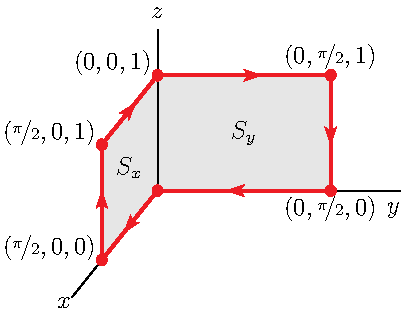
\includegraphics{OE05D_8.pdf}
\end{center}
}
We can choose the surface $S$ to be the union of two flat parts:
\begin{itemize}\itemsep1pt \parskip0pt \parsep0pt %\itemindent-15pt
\item[$\circ$]
the rectangle $S_x$ in the $xz$-plane with vertices $(0,0,0)$,
$(\nicefrac{\pi}{2},0,0)$, $(\nicefrac{\pi}{2},0,1)$ and $(0,0,1)$ and
\item[$\circ$]
the rectangle $S_y$ in the $yz$-plane with vertices $(0,0,0)$,
$(0,0,1)$, $(0,\nicefrac{\pi}{2},1)$ and $(0,\nicefrac{\pi}{2},0)$
\end{itemize} 
The normal to $S_x$ is $-\hj$ and the normal to $S_y$ is $-\hi$. Then Stokes'
theorem gives
\begin{align*}
\int_C\vF\cdot\dee{\vr}
&=\dblInt_S  \vnabla\times\vF\cdot\hn\,\dee{S} \\
&=\dblInt_{S_x}  \vnabla\times\vF\cdot(-\hj)\,\dee{S} 
  + \dblInt_{S_y}  \vnabla\times\vF\cdot(-\hi)\,\dee{S} \\
&=\int_0^{\nicefrac{\pi}{2}} \dee{x}\int_0^1\dee{z}\ z^2  
  + \int_0^{\nicefrac{\pi}{2}} \dee{y}\int_0^1\dee{z}\ z^2  \\
&=\int_0^{\nicefrac{\pi}{2}} \dee{x}\ \frac{1}{3}  
  + \int_0^{\nicefrac{\pi}{2}} \dee{y}\ \frac{1}{3}  \\
&=\frac{\pi}{3}
\end{align*}

\end{solution}

%%%%%%%%%%%%%%%%%%%%%%%%%%%%%%%
\begin{question}[M317 2017D] %4
Let
\begin{equation*}
\vF=\left(\frac{2z}{1+y}+\sin(x^2)\,,\,
           \frac{3z}{1+x}+\sin(y^2)\,,\,
           5(x+1)(y+2)\right)
\end{equation*}
Let $C$ be the oriented curve consisting of four line segments 
from $(0,0,0)$ to $(2,0,0)$,
from $(2,0,0)$ to $(0,0,2)$,
from $(0,0,2)$ to $(0,3,0)$, and
from $(0,3,0)$ to $(0,0,0)$.

\begin{enumerate}[(a)]
\item
Draw a picture of $C$. Clearly indicate the orientation
on each line segment.

\item
Compute the work integral $\int_C\vF\cdot\dee{\vr}$.
\end{enumerate}
\end{question}

%\begin{hint} 
%\end{hint}

\begin{answer} 
(a) 

\begin{center}
     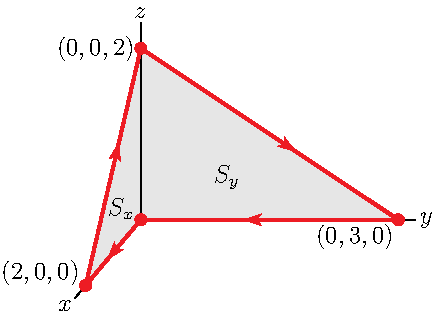
\includegraphics{OE17D_4.pdf}
\end{center}

(b) $\int_C\vF\cdot\dee{\vr} = 10$
\end{answer}

\begin{solution} (a) Here is a sketch.

\begin{center}
     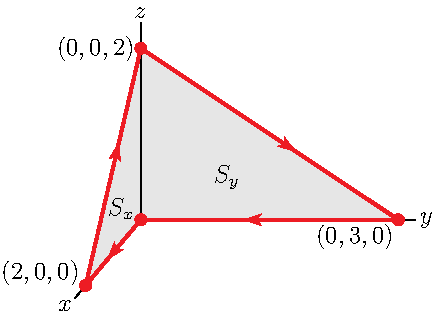
\includegraphics{OE17D_4.pdf}
\end{center}

(b) We are to evaluate the line integral of a complicated vector field
around a relatively complicated closed curve. That certainly suggests that
we should not try to evaluate the integral directly. Let's try
Stokes' theorem. First, we compute the curl
\begin{align*}
\vnabla\times\vF
&=\det\left[\begin{matrix}
\hi &\hj &\hk \\
\tfrac{\partial\hfill}{\partial x} & \tfrac{\partial\hfill}{\partial y} & 
                \tfrac{\partial\hfill}{\partial z} \\
       \frac{2z}{1+y}+\sin(x^2) & \frac{3z}{1+x}+\sin(y^2) & 5(x+1)(y+2)
       \end{matrix} \right] \\
&= \Big(5(x+1)-\frac{3}{1+x}\Big)\,\hi
  -\Big(5(y+2)-\frac{2}{1+y}\Big)\,\hj 
  +\Big(-\frac{3z}{(1+x)^2}+\frac{2z}{(1+y)^2}\Big)\,\hk
\end{align*}
Next we need to find a surface $S$ whose boundary is $C$.
We can choose the surface $S$ to be the union of two flat parts:
\begin{itemize}\itemsep1pt \parskip0pt \parsep0pt %\itemindent-15pt
\item[$\circ$]
the triangle $S_x$ in the $xz$-plane with vertices $(0,0,0)$,
$(2,0,0)$, and $(0,0,2)$ and
\item[$\circ$]
the triangle $S_y$ in the $yz$-plane with vertices $(0,0,0)$,
$(0,0,2)$, and $(0,3,0)$
\end{itemize} 
Note that
\begin{itemize}\itemsep1pt \parskip0pt \parsep0pt %\itemindent-15pt
\item[$\circ$]
The normal to $S_x$ specified by Stokes' theorem is $-\hj$. On $S_x$
we have $y=0$, so that $\vnabla\times\vF\cdot\hj$ simplifies to 
$-\big(5(0+2)-\frac{2}{1+0}\big)=-8$.
\item[$\circ$]
The normal to $S_y$ specified by Stokes' theorem is $-\hi$. On $S_y$
we have $x=0$, so that $\vnabla\times\vF\cdot\hi$ simplifies to 
$\big(5(0+1)-\frac{3}{1+0}\big)=2$.
\end{itemize} 
So Stokes' theorem gives
\begin{align*}
\int_C\vF\cdot\dee{\vr}
&=\dblInt_S  \vnabla\times\vF\cdot\hn\,\dee{S} 
=\dblInt_{S_x}  \overbrace{\vnabla\times\vF\cdot(-\hj)}^{8}\,\dee{S} 
  + \dblInt_{S_y}  \overbrace{\vnabla\times\vF\cdot(-\hi)}^{-2}\,\dee{S} \\
&=8\,\text{Area}(S_x)  -2\,\text{Area}(S_y)
  =8\frac{1}{2}(2)(2) -2\frac{1}{2}(3)(2) \\
&=10
\end{align*}
\end{solution}

%%%%%%%%%%%%%%%%%%%%%%%%%%%
\begin{question}[M317 2004A] %7
Evaluate $\displaystyle\dblInt_S\vnabla\times\vF\cdot\hn\,\dee{S}$ where
$\vF=y\,\hi+2z\,\hj+3x\,\hk$ and $S$ is the surface $z=\sqrt{1-x^2-y^2}$,
$z\ge 0$ and $\hn$ is a unit normal to $S$ obeying $\hn\cdot\hk\ge 0$.
\end{question}

%\begin{hint} 
%\end{hint}

\begin{answer} 
$-\pi$
\end{answer}


\begin{solution}
 The boundary, $\partial S$, of $S$ is the circle $x^2+y^2=1$
oriented counter clockwise as usual. It may be parametrized by
$\vr(\theta)=\cos\theta\,\hi+\sin\theta\hj$, $0\le\theta\le 2\pi$. By Stokes' theorem
\begin{align*}
\dblInt_S\vnabla\times\vF\cdot\hn\,\dee{S}
&=\oint_{\partial S} \vF\cdot\dee{\vr}
=\int_0^{2\pi}\vF\big(\vr(\theta)\big)\cdot\diff{\vr}{\theta}(\theta)
       \,\dee{\theta} \\
& =\int_0^{2\pi}(\sin\theta,0,3\cos\theta)\cdot(-\sin\theta,\cos\theta,0)
        \,\dee{\theta} \\
&=-\int_0^{2\pi}\sin^2\theta\,\dee{\theta}
=-\int_0^{2\pi}\dee{\theta}\,\frac{1-\cos(2\theta)}{2}
=-\left[\frac{\theta}{2}-\frac{\sin(2\theta)}{4}\right]_0^{2\pi} \\
&=-\pi
\end{align*}
For an efficient, sneaky, way to evaluate 
$\int_0^{2\pi}\dee{\theta}\ \sin^2\theta$, see Example
\eref{CLP317}{eg:workIntegalB} in the CLP-4 text.
\end{solution}


%%%%%%%%%%%%%%%%%%%%%%%%%%%
\begin{question}[M317 2000D] %4
Let $\cS$ be the curved surface below, oriented by the outward normal:
$$
x^2 + y^2 + 2(z-1)^2 = 6,\qquad z\ge 0.
$$
(E.g., at the high point of the surface, the unit normal is $\hk$.) 
%\hfill\break
Define 
$$
\vG = \nabla\times\vF,
\qquad{\rm where}\qquad
\vF = (xz - y^3\cos z)\,\hi + x^3 e^z\,\hj + xyze^{x^2+y^2+z^2}\,\hk.
$$
Find $\dblInt_\cS \vG\cdot \hn\dee{S}$.

\end{question}

%\begin{hint} 
%\end{hint}

\begin{answer} 
$24\pi$
\end{answer}


\begin{solution}
The given surface is an ellipsoid centred at $(x,y,z)=(0,0,1)$.
It caps a curve $\cC$ in the plane $z=0$, given by $x^2+y^2=4$.
This is a circle of radius $2$ centred at the origin, oriented
counterclockwise when viewed from the positive $z$-axis.

\emph{Method I --- double Stokes':}\ \ \ 
Let $\cD$ denote the plane disk $x^2+y^2\le 4$, $z=0$.
Using Stokes' theorem twice gives
$$
\dblInt_\cS \vG\cdot \hn\,\dee{S}
= \dblInt_\cS \nabla\times\vF\cdot \hn\,\dee{S}
= \oint_\cC \vF\cdot \dee{\vr}
= \dblInt_\cD \nabla\times\vF\cdot \hn\,\dee{S}
= \dblInt_\cD \vG\cdot \hn\,\dee{S}
$$
Now in $\cD$ we have $\hn=\hk$ and $z=0$, so on this surface,
\begin{align*}
\vG\cdot\hn
= (\nabla\times\vF)\cdot\hk
&= \det\left[\begin{matrix} 0 & 0 & 1 \\
\frac{\partial\hfill}{\partial x} & \frac{\partial\hfill}{\partial y} & \frac{\partial\hfill}{\partial z} \\
(xz - y^3\cos z) & x^3 e^z & xyze^{x^2+y^2+z^2} \end{matrix}\right]_{z=0}
\\[0.05in]
&= \big[3x^2 e^z + 3y^2\cos z\big]_{z=0}
= 3(x^2+y^2)
\end{align*}
Hence, using polar coordinates,
$$
\dblInt_\cS \vG\cdot \hn\,\dee{S}
= \dblInt_\cD 3(x^2+y^2)\,\dee{x}\dee{y}
= 3\int_{\theta=0}^{2\pi} \int_{r=0}^2 (r^2)\,r\,\dee{r}\,\dee{\theta}
= 3(2\pi)(4)= 24\pi
$$

\emph{Method II --- single Stokes':}\ \ \ 
By Stokes' theorem
\begin{equation*}
\dblInt_\cS \vG\cdot \hn\,\dee{S}
= \dblInt_\cS \nabla\times\vF\cdot \hn\,\dee{S}
= \oint_\cC \vF\cdot \dee{\vr}
\end{equation*}
Parametrize the circle $\cC$ using
$$
\vr(\theta) = 2\cos\theta\,\hi + 2\sin\theta\,\hj,\qquad 0\le\theta\le 2\pi
$$
to obtain
$$
\dee{\vr} = \diff{\vr}{\theta}\,\dee{\theta}
= (-2\sin\theta\,\hi + 2\cos\theta\,\hj)\,\dee{\theta}.
$$
Then since $z=0$ on $\cC$,
\begin{align*}
\dblInt_\cS \vG\cdot \hn\,\dee{S}
&= \int_{0}^{2\pi}\big(
\overbrace{-(2\sin\theta)^3\,\hi + (2\cos\theta)^3\,\hj}^
                                          {\vF\big(\vr(\theta)\big)}\big)
\cdot \big(\overbrace{-2\sin\theta\,\hi + 2\cos\theta\,\hj}^{\vr'(\theta)}\big)
 \,\dee{\theta}
\\
&= 16 \int_{0}^{2\pi}\big(\sin^4\theta + \cos^4\theta\big)\,\dee{\theta}
%= 32 \int_{0}^{2\pi} \sin^4\theta\,\dee{\theta}
%= 64 \int_{0}^{\pi} \sin^4\theta\,\dee{\theta}
\end{align*}
By the double angle trig identities
\begin{align*}
\cos^2\theta=\frac{1+\cos(2\theta)}{2}\qquad
\sin^2\theta=\frac{1-\cos(2\theta)}{2}\qquad
\end{align*}
we have
\begin{align*}
\sin^4\theta + \cos^4\theta
&=\frac{\big[1-\cos(2\theta)\big]^2}{4} 
 + \frac{\big[1+\cos(2\theta)\big]^2}{4} \\
&=\frac{1}{2} + \frac{\cos^2(2\theta)}{2}
=\frac{1}{2} + \frac{1+\cos(4\theta)}{4}
\end{align*}
So
$$
\dblInt_\cS \vG\cdot \hn\,\dee{S}
=16\int_{0}^{2\pi} \left(\frac{3}{4}+\frac{1}{4}\cos(4\theta)\right)
                   \,\dee{\theta}
= 16\times\frac{3}{4}\times (2\pi) = 24\pi
$$

\end{solution}

%%%%%%%%%%%%%%%%%%%%%%%%%%%
\begin{question}[M317 1999A] %6
 Let $C$ be a circle of radius $R$ lying in the plane $x+y+z=3$.
Use Stokes' Theorem to calculate the value of 
$$
\oint_C \vF\cdot \dee{\vr}
$$
where $\vF=z^2\hi+x^2\hj+y^2\hk$. (You may use either orientation of the
circle.)

\end{question}

\begin{hint} 
Let $D$ be the disk in the plane $x+y+z=3$ whose boundary is $C$.
Suppose that, as $(x,y,z)$ runs over $D$, $(x,y)$ runs over the
ellipse $D_{xy}$. 
We are told that the area of $D$ is $\pi R^2$, but we are
not told the area of $D'$. So it is easier to deal with the
integral $\dblInt_D \dee{S}$ than with the integral 
$\dblInt_{D'}\dee{x}\dee{y}$.
\end{hint}

\begin{answer} 
$2\sqrt{3}\pi R^2$
\end{answer}


\begin{solution}
Note that
$$
\vnabla\times\vF=\det\left|\begin{matrix}\hi&\hj&\hk\\[0.03in] \frac{\partial\hfill}{\partial x}&
        \frac{\partial\hfill}{\partial y}&
        \frac{\partial\hfill}{\partial z}\\[0.03in]
z^2&x^2&y^2\end{matrix}\right|
=2y\,\hi+2z\,\hj+2x\,\hk
$$
Let $D$ be the disk in the plane $x+y+z=3$ whose boundary is $C$ and let
$\hn=\frac{1}{\sqrt{3}}(\hi+\hj+\hk)$ be the upward unit normal to $D$.
If the circle is oriented counterclockwise, when viewed from above,
then, by Stokes' theorem  (Theorem \eref{CLP317}{thm:Stokes} in the CLP-4 text),
\begin{align*}
\oint_C \vF\cdot \dee{\vr}
&=\dblInt_D \vnabla\times\vF\cdot\hn\ \dee{S}
=\frac{1}{\sqrt{3}}
\dblInt_D \big(2y\,\hi+2z\,\hj+2x\,\hk\big)\cdot(\hi+\hj+\hk)\ \dee{S}\\
&=\frac{1}{\sqrt{3}}\dblInt_D2\overbrace{\big(x+y+z\big)}^{=3\text{ on $D$}}\ \dee{S}
=2\sqrt{3}\dblInt_D \dee{S}
=2\sqrt{3}\pi R^2
\end{align*}
\end{solution}

%%%%%%%%%%%%%%%%%%%%%%%%%%%%%%%
\begin{question}
Let $S$ be the oriented surface consisting of the top and
four sides of the cube whose vertices are $(\pm 1,\pm1,\pm1)$, oriented
outward. If $\vF(x,y,z)=(xyz,xy^2,x^2yz)$, find the flux of 
$\vnabla\times\vF$ through $S$.
\end{question}

%\begin{hint} 
%\end{hint}

\begin{answer} 
$\frac{4}{3}$
\end{answer}

\begin{solution} \emph{Solution 1}:\ \ \ 
Let $S'$ be the bottom surface of the cube, oriented with
normal $\hk$. Then, by Stokes' theorem, since $\partial S=\partial S'$,
\begin{equation*}
\dblInt_S\vnabla\times\vF\cdot\hn\, \dee{S}
=\oint_{\partial S}\vF\cdot \dee{\vr}
=\oint_{\partial S'}\vF\cdot \dee{\vr}
=\dblInt_{S'}\vnabla\times\vF\cdot\hn\, \dee{S}
\end{equation*}
Since 
\begin{align*}
\vnabla\times\vF=\det\left[\begin{matrix}\hi & \hj & \hk \\[0.05in]
                  \pdiff{}{x} &
                  \pdiff{}{y} &
                  \pdiff{}{z} \\[0.05in]
                  xyz & xy^2 & x^2yz \end{matrix}\right] 
=\big(\cdots\,,\,\cdots\,,\,y^2-xz\big)
\end{align*}
and $\hn=\hk$ on $S'$ and $z=-1$ on $S'$
\begin{align*}
\dblInt_{S'}\vnabla\times\vF\cdot\hn\, \dee{S}
&=\int_{-1}^1 \dee{x}\int_{-1}^1 \dee{y}\ 
         \big(\cdots,\cdots,y^2-xz\big)\cdot\hk\Big|_{z=-1}
=\int_{-1}^1 \dee{x}\int_{-1}^1 \dee{y}\  (y^2+x) \\
&=\int_{-1}^1 \dee{x}\int_{-1}^1 \dee{y}\  y^2
=2\times 2\int_0^1\dee{y}\ y^2
=\frac{4}{3}
\end{align*}


\emph{Solution 2}:\ \ \ 
The boundary of $S$ is the square $C$, with sides $C_1$, $\cdots$, $C_4$, 
in the sketch
\begin{center}
       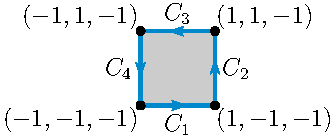
\includegraphics{cubeS.pdf}
\end{center}
By Stokes' theorem,
\begin{equation*}
\dblInt_S\vnabla\times\vF\cdot\hn\, \dee{S}
=\oint_{C}\vF\cdot \dee{\vr}
\end{equation*}
Parametrize $C_1$ by $x$. That is, $\vr(x)= x\hi - \hj -\hk$, $-1\le x\le 1$.
Since $\vr'(x) = \hi$, and $y=z=-1$ on $C_1$,
\begin{align*}
\int_{C_1}\vF\cdot \dee{\vr}
&=\int_{-1}^1 \vF\big(\vr(x)\big)\cdot\vr'(x)\ \dee{x}
=\int_{-1}^1 \vF\big(\vr(x)\big)\cdot\hi\ \dee{x}
=\int_{-1}^1\overbrace{x(-1)(-1)}^{xyz}\ \dee{x} \\
&=0\qquad\text{(since $x$ is odd)}
\end{align*}
Parametrize $C_2$ by $y$. That is, $\vr(y)= \hi + y\,\hj -\hk$, $-1\le y\le 1$.
Since $\vr'(y) = \hj$, and $x=1$ on $C_2$,
\begin{align*}
\int_{C_2}\vF\cdot \dee{\vr}
=\int_{-1}^1 \vF\big(\vr(y)\big)\cdot\hj\ \dee{y}
=\int_{-1}^1\overbrace{y^2}^{xy^2}\ \dee{y}
=\left[\frac{y^3}{3}\right]_{-1}^1
=\frac{2}{3}
\end{align*}
Parametrize $C_3$ by $x$. That is, $\vr(x)= x\hi + \hj -\hk$ with $x$ running
from $1$ to $-1$. (If you're nervous about this, parametrize
by $t=-x$. That is $\vr(t)= -t\,\hi + \hj -\hk$, $-1\le t\le 1$.)
Since $\vr'(x) = \hi$, and $y=1$, $z=-1$ on $C_3$,
\begin{align*}
\int_{C_3}\vF\cdot \dee{\vr}
=\int^{-1}_1 \vF\big(\vr(x)\big)\cdot\hi\ \dee{x}
=\int^{-1}_1\overbrace{x\ (1)(-1)}^{xyz}\ \dee{x}
=0\qquad\text{(since $x$ is odd)}
\end{align*}
Parametrize $C_4$ by $y$. That is, $\vr(y)= -\hi + y\,\hj -\hk$, with
$y$ running from $1$ to $-1$. Since $\vr'(y) = \hj$, and $x=-1$ on $C_4$,
\begin{align*}
\int_{C_4}\vF\cdot \dee{\vr}
=\int^{-1}_1 \vF\big(\vr(y)\big)\cdot\hj\ \dee{y}
=\int^{-1}_1\overbrace{(-1)y^2}^{xy^2}\ \dee{y}
=-\left[\frac{y^3}{3}\right]^{-1}_1
=\frac{2}{3}
\end{align*}
All together
\begin{equation*}
\dblInt_S\vnabla\times\vF\cdot\hn\, \dee{S}
=\int_{C_1}\vF\cdot \dee{\vr} + \int_{C_2}\vF\cdot \dee{\vr}
 +\int_{C_3}\vF\cdot \dee{\vr} + \int_{C_4}\vF\cdot \dee{\vr}
=\frac{4}{3}
\end{equation*}
\end{solution}

%%%%%%%%%%%%%%%%%%%%%%%%%%%%%%%
\begin{question}
Let $S$ denote the part of the spiral ramp (that is helicoidal
surface) parametrized by 
\begin{equation*}
x=u\cos v,\ y=u\sin v,\ z=v\qquad
0\le u\le 1,\ 0\le v\le 2\pi
\end{equation*}
Let $C$ denote the boundary of $S$
with orientation specified by the upward pointing normal on $S$. Find
\begin{equation*}
\int_C y\,\dee{x}-x\,\dee{y}+ xy\,\dee{z}
\end{equation*}
\end{question}

%\begin{hint} 
%\end{hint}

\begin{answer} 
$-2\pi$
\end{answer}

\begin{solution} 
Let's try Stokes' Theorem. Call $\vF=y\,\hi-x\,\hj+xy\,\hk$. Then
\begin{align*}
\vnabla\times\vF=\det\left[\begin{matrix}\hi & \hj & \hk \\[0.05in]
                  \pdiff{}{x} &
                  \pdiff{}{y} &
                  \pdiff{}{z} \\[0.05in]
                  y & -x & xy \end{matrix}\right] 
=x\,\hi-y\,\hj-2\,\hk
\end{align*}
Now compute $\hn\,\dee{S}$ in the $(u,v)$-parametrization.
\begin{align*}
\vr(u,v)&=\big(u\cos v, u\sin v, v\big)\\
\pdiff{\vr}{u}(u,v)&=\big(\cos v, \sin v, 0\big)\\
\pdiff{\vr}{v}(u,v)&=\big(-u\sin v, u\cos v, 1\big)\\
\pdiff{\vr}{u}\times\pdiff{\vr}{v}
&=\det\left[\begin{matrix}\hi & \hj & \hk \\[0.05in]
                  \cos v & \sin v & 0 \\
                  -u\sin v& u\cos v& 1 \end{matrix}\right] 
=\big(\sin v, -\cos v, u\big)\\
\hn\,\dee{S}&=\big(\sin v, -\cos v, u\big)\,\dee{u}\,\dee{v}
\end{align*}
Since $u\ge 0$, we do indeed have the upward pointing normal.
So, Stokes' theorem tells us
\begin{align*}
\int_C y\,\dee{x}-x\,\dee{y}+ xy\,\dee{z}
&=\int_C\vF\cdot \dee{\vr}
=\dblInt_S \vnabla\times\vF\cdot\hn\,\dee{S}\\
&=\int_0^1 \dee{u} \int_0^{2\pi} \dee{v}\  \big(u\cos v, -u\sin v, -2\big)
\cdot\big(\sin v, -\cos v, u\big)\\
&=\int_0^1 \dee{u} \int_0^{2\pi} \dee{v}\ \big(2u\sin v\cos v-2u\big)
=\left[\int_0^1 \dee{u} \ u\right]
    \left[\int_0^{2\pi} \dee{v}\ \big(\sin 2v-2\big)\right]\\
&=\half(-4\pi)=-2\pi
\end{align*}
\end{solution}





%%%%%%%%%%%%%%%%%%
\subsection*{\Application}
%%%%%%%%%%%%%%%%%%

%%%%%%%%%%%%%%%%%%%%%%%%%%%%%%%
\begin{question}
Let $C$ be the intersection of $x+2y-z=7$ and $x^2-2x+4y^2=15$.
The curve $C$ is oriented counterclockwise when viewed from high on the
$z$-axis. Let
\begin{equation*}
\vF=\big(e^{x^2}+yz\big)\,\hi
   +\big(\cos(y^2)-x^2\big)\,\hj
   +\big(\sin(z^2)+xy\big)\,\hk
\end{equation*}
Evaluate $\oint_C\vF\cdot \dee{\vr}$.
\end{question}

\begin{hint} 
Given the form of $\vF$, direct evaluation looks hard.

The integral evaluations can be greatly simplified by using
that the centroid $(\bar x,\bar y)$ of any region $R$ in the $xy$-plane
is
\begin{equation*}
\bar x =\frac{\dblInt_R x\,\dee{x}\,\dee{y}}{\text{Area}(R)}\qquad
\bar y =\frac{\dblInt_R y\,\dee{x}\,\dee{y}}{\text{Area}(R)}
\end{equation*}

\end{hint}

\begin{answer} 
$24\pi$
\end{answer}

\begin{solution} 
Given the form of $\vF$, direct evaluation looks hard. So let's try
Stokes' theorem, using as $S$ the part of the plane $G(x,y,z)=x+2y-z=7$ 
that is inside $x^2-2x+4y^2=15$. Then
\begin{equation*}
\hn\,\dee{S} = \pm \frac{\vnabla G}{\vnabla G\cdot\hk}\,\dee{x}\,\dee{y}
= \pm\big(\hi+2\hj-\hk\big)\,\dee{x}\,\dee{y}
\end{equation*} 
As $C$ is oriented counterclockwise when viewed from high, Stokes'
theorem specifies the upward pointing normal so that 
$\hn\,\dee{S} = -\big(\hi+2\hj-\hk\big)\,\dee{x}\,\dee{y}$.

From the observations that 
\begin{equation*}
\vnabla\times\vF=\det\left[\begin{matrix}\hi & \hj & \hk \\[0.05in]
                  \pdiff{}{x} &
                  \pdiff{}{y} &
                  \pdiff{}{z} \\[0.05in]
                  e^{x^2}+yz & \cos(y^2)-x^2 & \sin(z^2)+xy
                  \end{matrix} \right] 
=x\,\hi-(z+2x)\,\hk
\end{equation*}
and that we can rewrite $x^2-2x+4y^2=15$ as $(x-1)^2+4y^2=16$,
we have
\begin{align*}
\oint_C\vF\cdot \dee{\vr}
&=\dblInt_S \vnabla\times\vF\cdot\hn\,\dee{S}\\
&=\dblInt_{(x-1)^2+4y^2\le 16}\,
     [x\hi-(z+2x)\hk]\Big|_{z=-7+x+2y}\cdot(-1,-2,1)\,\dee{x}\,\dee{y}\\
&=\dblInt_{(x-1)^2+4y^2\le 16} [-x-(-7+x+2y+2x)]\,\dee{x}\,\dee{y}\\
&=\dblInt_{(x-1)^2+4y^2\le 16} [7-4x-2y]\,\dee{x}\,\dee{y}
\end{align*}
To evaluate the integrals of $x$ and $y$ we use that, for any region $R$
in the $xy$--plane,
\begin{equation*}
\bar x =\frac{\dblInt_R x\,\dee{x}\,\dee{y}}{\text{Area}(R)}\qquad
\bar y =\frac{\dblInt_R y\,\dee{x}\,\dee{y}}{\text{Area}(R)}
\end{equation*}
Our ellipse is $\frac{(x-1)^2}{4^2}+\frac{y^2}{2^2}=1$ 
and so has area $\pi ab = \pi\times4\times 2=8\pi$ and centroid
$(\bar x,\bar y) = (1,0)$. So, using
$R=\Set{(x,y)}{\frac{(x-1)^2}{4^2}+\frac{y^2}{2^2}\le 1}$, 
\begin{align*}
\oint_C\vF\cdot \dee{\vr}
&=\dblInt_R [7-4x-2y]\,\dee{x}\,\dee{y}\\
&=\text{Area}(R) \big\{7-4\bar x-2\bar y\}\\
&=8\pi[7-4\times 1-2\times 0]=24\pi
\end{align*}
\end{solution}

%%%%%%%%%%%%%%%%%%%%%%%%%%%
\begin{question}[M317 2012D] %4
\begin{enumerate}[(a)]
\item
Find the curl of the vector field 
$\vF  = \big(2 + x^2 + z\,,\, 0\,,\, 3 + x^2 z\big)$.
\item
Let $C$ be the curve in $\bbbr^3$ from the point $(0, 0, 0)$ to 
the point $(2, 0, 0)$, consisting of three consecutive line segments 
connecting the points $(0, 0, 0)$ to $(0, 0, 3)$,
$(0, 0, 3)$ to $(0, 1, 0)$, and $(0, 1, 0)$ to $(2, 0, 0)$. 
Evaluate the line integral
\begin{equation*}
\int_C \vF\cdot\dee{\vr} 
\end{equation*}
where $\vF$ is the vector field from (a).
\end{enumerate}
\end{question}

\begin{hint} 
Part (a) is a hint for part (b). Sketch the curve in part (b).
\end{hint}

\begin{answer} 
(a) $\vnabla\times\vF=(1-2xz)\,\hj$\qquad
(b) $\nicefrac{20}{3}$
\end{answer}


\begin{solution}
(a) 
The curl is
\begin{align*}
\vnabla\times\vF
&=\det\left[\begin{matrix}
\hi &\hj &\hk \\
\tfrac{\partial\hfill}{\partial x} & \tfrac{\partial\hfill}{\partial y} & 
                \tfrac{\partial\hfill}{\partial z} \\
2+x^2+z &  0 & 3+x^2z
\end{matrix}
\right]
=(1-2xz)\,\hj
\end{align*}

\noindent (b) We are going to use Stokes' theorem. The specified curve $C$
is not closed and so is not the boundary of a surface. So we extend
$C$ to a closed curve $\tilde C$ by appending to $C$ the line segment $L$
from $(2,0,0)$ to $(0,0,0)$. In the figure below, $C$ is the red curve 
and $\tilde C$ is $C$ plus the blue line segment. 
\vadjust{
\begin{center}
       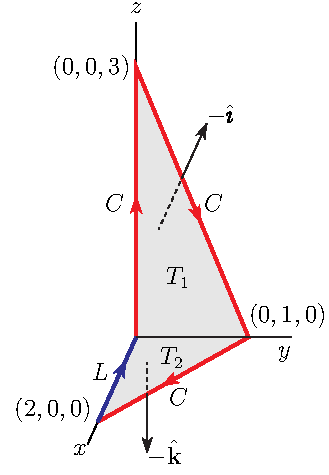
\includegraphics[scale=0.9]{OE12D_4.pdf}
\end{center}
}
The closed curve $\tilde C$ is boundary of the surface $S$ that is the
union of 
\begin{itemize}\itemsep1pt \parskip0pt \parsep0pt %\itemindent-15pt
\item[$\circ$] the triangle $T_1$ in the $yz$-plane
with vertices $(0,0,0)$, $(0,0,3)$ and $(0,1,0)$ 
and with normal vector $-\hi$ and
\item[$\circ$] the triangle $T_2$ in the $xy$-plane 
with vertices $(0,0,0)$, $(0,1,0)$ and $(2,0,0)$ 
and with normal vector $-\hk$.
\end{itemize}
So, by Stokes' theorem
\begin{align*}
\int_C \vF\cdot\dee{\vr} + \int_L \vF\cdot\dee{\vr}
&=  \int_{\partial S} \vF\cdot\dee{\vr}  
= \dblInt_S \vnabla\times \vF\cdot\hn\,\dee{S} \\ 
&= \dblInt_{T_1} \vnabla\times \vF\cdot(-\hi)\,\dee{S}
  + \dblInt_{T_2} \vnabla\times \vF\cdot(-\hk)\,\dee{S} \\ 
&= \dblInt_{T_1} (1-2xz)\,\hj\cdot(-\hi)\,\dee{S}
  + \dblInt_{T_2} (1-2xz)\,\hj\cdot(-\hk)\,\dee{S} \\ 
&=0
\end{align*}
Consequently the integral of interest
\begin{align*}
\int_C \vF\cdot\dee{\vr}
&=- \int_L \vF\cdot\dee{\vr}
=- \int_2^0 (2+x^2)\,\dee{x}
\qquad\text{since $\dee{y}=\dee{z}=z=0$ on $L$} \\
&=\int_0^2 (2+x^2)\,\dee{x}
={\left[2x+\frac{x^3}{3}\right]}_0^2
=\frac{20}{3}
\end{align*}
\end{solution}

%%%%%%%%%%%%%%%%%%%%%%%%%%%
\begin{question}[M317 2012D] %6
\begin{enumerate}[(a)]
\item
Let $S$ be the bucket shaped surface consisting of the cylindrical surface 
$y^2 + z^2 = 9$ between $x = 0$ and $x = 5$, and the disc inside the 
$yz$-plane of radius $3$ centered at the origin. (The bucket $S$ 
has a bottom, but no lid.) Orient $S$ in such a way that the unit normal 
points outward. Compute the flux of the vector field $\vnabla\times\vG$
through $S$, where $\vG = (x, -z, y)$.
\item
Compute the flux of the vector field $\vF = (2 + z, xz^2 , x \cos y)$ 
through $S$, where $S$ is as in (a).
\end{enumerate}
\end{question}

\begin{hint} 
For practice, evaluate the flux of part (a) twice --- once by direct
evaluation and once using Stokes' theorem.
\end{hint}

\begin{answer} 
(a) $-18\pi$ \qquad
(b) $-18\pi$
\end{answer}


\begin{solution}
(a) \emph{by direct evaluation:}\ \ \ 
The curl of $\vG$ is
\begin{align*}
\vnabla\times\vG
&=\det\left[\begin{matrix}
\hi &\hj &\hk \\
\tfrac{\partial\hfill}{\partial x} & \tfrac{\partial\hfill}{\partial y} & 
                \tfrac{\partial\hfill}{\partial z} \\
x & -z & y
\end{matrix}
\right]
=2\hi
\end{align*}
The part of $S$ in the first octant is sketched in the figure on the left below.
$S$ consists of two parts --- the cylindrical surface
\begin{equation*}
S_1 = \Set{(x,y,z)}{y^2+z^2=9,\ 0\le x\le 5}
\end{equation*}
and the disc
\begin{equation*}
S_2 = \Set{(x,y,z)}{x=0,\ y^2+z^2\le 9}
\end{equation*}
The normal $\hn$ to $S_1$ always points radially outward from the cylinder
and so always has $\hi$ component zero. The normal of $S_2$ is $-\hi$.
So the flux is
\begin{align*}
\dblInt_S \vnabla\times \vG \cdot \hn\,\dee{S}
&= \dblInt_{S_1} 2\hi \cdot \hn\,\dee{S}
   + \dblInt_{S_2} 2\hi \cdot (-\hi)\,\dee{S} \\
&= -2 \dblInt_{S_2} \dee{S} \\
&= -2 \big(\pi 3^2\big) = -18\pi
\end{align*}



(a) \emph{using Stokes' theorem:}\ \ \ 
Let's use Stokes' theorem. The boundary $\partial S$ of $S$ is the cirlce 
$y^2+z^2=9$, $x=5$, oriented clockwise when viewed from far down the $x$-axis.
We'll parametrize it by $\vr(\theta)=\big(5, 3\cos\theta, -3\sin\theta\big)$.
Then Stokes' theorem gives
\begin{align*}
\dblInt_S \vnabla\times\vG\cdot\hn\,\dee{S}
&=\oint_{\partial S}\vG\cdot\dee{\vr} \\
&=\int_0^{2\pi} \big(5\,,\,3\sin\theta,3\cos\theta\big)\cdot
       \big(0\,,\,-3\sin\theta\,,\,-3\cos\theta\big)\,\dee{\theta} \\
&=\int_0^{2\pi} \big(-9\sin^2\theta-9\cos^2\theta\big)\,\dee{\theta} \\
&=-18\pi
\end{align*} 

\begin{center}
       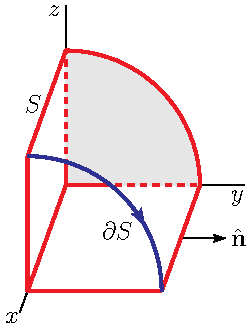
\includegraphics{OE12D_6a.pdf} \qquad\qquad
       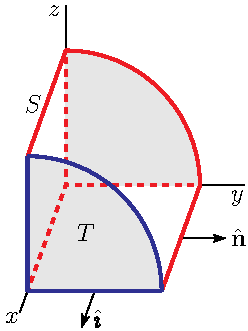
\includegraphics{OE12D_6b.pdf}
\end{center}

\noindent (b)
This time we'll use the divergence theorem. The surface $S$ is not closed.
So we'll use the auxilary surface formed by ``topping $S$ off''
with the cap $T=\Set{(5,y,z)}{y^2+z^2\le 9}$. If we give $T$ the normal vector $\hi$, this auxiliary surface, the union of $S$ and $T$, is the boundary of 
$V=\Set{(x,y,z)}{y^2+z^2\le 9,\ 0\le x\le 5}$. So the divergence theorem gives
\begin{align*}
\dblInt_S  \vF\cdot\hn\,\dee{S}
+\dblInt_T \vF\cdot\hn\,\dee{S} 
&= \dblInt_{\partial V} \vF\cdot\hn\,\dee{S} \\
&=\tripInt_V \vnabla\cdot \vF\ \dee{V} \\
&=0
\end{align*}
since $\vnabla\cdot \vF = 0$. Thus the flux of interest is
\begin{align*}
\dblInt_S  \vF\cdot\hn\,\dee{S}
&=-\dblInt_T \vF\cdot\hn\,\dee{S} 
=-\dblInt_T \vF\cdot\hi\,\dee{S} 
=-\dblInt_T (2+z)\,\dee{S} \\
&=-2\dblInt_T \,\dee{S} 
   \qquad\text{since $\dblInt_T z\,\dee{S}=0$, because $z$ is odd}\\
&= -18\pi
    \qquad\text{since $T$ has area $9\pi$}
\end{align*}
\end{solution}

%%%%%%%%%%%%%%%%%%%%%%%%%%%
\begin{question}[M317 2010D] %5
Let
\begin{equation*}
\vF(x, y, z) = \Big(\frac{y}{x} +x^{1+x^2}\,,\, x^2-y^{1+y^2}\,,\,
                       \cos^5(\ln z)\Big)
\end{equation*}
\begin{enumerate}[(a)]
\item
Write down the domain $D$ of $\vF$.

\item
Circle the correct statement(s):
\begin{enumerate}[(a)]
\item D is connected.
\item D is simply connected.
\item D is disconnected.
\end{enumerate}

\item 
Compute $\vnabla\times\vF$.

\item 
Let $C$ be the square with corners $(3 \pm 1, 3 \pm 1)$ in the plane 
$z = 2$, oriented clockwise (viewed from above, i.e. down $z$-axis). 
Compute 
\begin{equation*}
\int_C \vF \cdot \dee{\vr}
\end{equation*}

\item
Is $\vF$ conservative?

\end{enumerate}
\end{question}

\begin{hint} 
By definition, $D$ is connected if any two points in $D$
can be joined by a curve that lies completely in $D$.


By definition, $D$ is simply connected if any simple closed curve in 
$D$ can be shrunk to a point continuously in $D$.
\end{hint}

\begin{answer} 
(a) $D=\Set{(x,y,z)}{x>0,\ y>0,\ z>0}$

(b) The domain $D$ is both connected and simply connected.

(c) $\vnabla\times\vF=\big(2x-\nicefrac{1}{x}\big)\hk$

(d) $2\ln 2-24$

(e) No. $\vF$ is not conservative.
\end{answer}


\begin{solution}
(a)
Since 
\begin{itemize}\itemsep1pt \parskip0pt \parsep0pt %\itemindent-15pt
\item[$\circ$]
$\frac{y}{x}$ is defined when $x\ne 0$ and
\item[$\circ$]
$x^{1+x^2}=e^{(1+x^2)\ln x}$ is defined when $\ln x$ is defined, 
which is when $x>0$ (assuming that we are not allowed to use complex numbers)
and
\item[$\circ$]
$y^{1+y^2}=e^{(1+y^2)\ln y}$ is defined when $\ln y$ is defined, 
which is when $y>0$ and
\item[$\circ$]
$\cos^5(\ln z)$ is defined when $\ln z$ is defined, 
which when $z>0$
\end{itemize}
the domain of $\vF$ is
\begin{equation*}
D=\Set{(x,y,z)}{x>0,\ y>0,\ z>0}
\end{equation*}

\noindent (b) The domain $D$ is both connected (any two points in $D$
can be joined by a curve that lies completely in $D$) and 
simply connected (any simple closed curve in $D$ can be shrunk to a 
point continuously in $D$).


\noindent (c) The curl of $\vF$ is 
\begin{align*}
\vnabla\times\vF
&=\det\left[\begin{matrix}
\hi &\hj &\hk \\
\tfrac{\partial\hfill}{\partial x} & \tfrac{\partial\hfill}{\partial y} & 
                \tfrac{\partial\hfill}{\partial z} \\
\frac{y}{x} +x^{1+x^2} & x^2-y^{1+y^2} & \cos^5(\ln z)
\end{matrix}
\right]
=\big(2x-\nicefrac{1}{x}\big)\hk
\end{align*}

\noindent (d) 
The integrand for direct evaluation looks very complicated.
On the other hand $\vnabla\times\vF$ is quite simple. So let's
try Stokes' thoerem.
Denote 
\begin{equation*}
S=\Set{(x,y,z)}{2\le x\le 4,\ 2\le y\le 4,\ z=2}
\end{equation*}
The boundary of $S$ is $C$. Because of the clockwise orientation
of $C$, we assign the normal vector $-\hk$ to $S$. See the sketch below

\begin{center}
       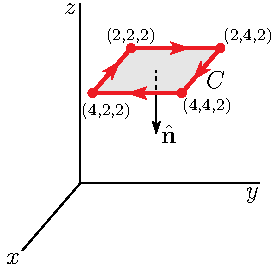
\includegraphics{OE10D_5.pdf}
\end{center}


\noindent
Then, by Stokes'
theorem,
\begin{align*}
\oint_C\vF\cdot\dee{\vr}
&=\dblInt_S \vnabla\times\vF\cdot\hn\,\dee{S} 
= \dblInt_S \vnabla\times\vF\cdot(-\hk)\,\dee{S}
= -\dblInt_S \big(2x-\tfrac{1}{x}\big)\,\dee{S}  \\
&= -\int_2^4\dee{x}\int_2^4\dee{y}\ \big(2x-\tfrac{1}{x}\big)
 =-\int_2^4\dee{x}\ 2\big(2x-\tfrac{1}{x}\big)
 = - 2\Big[x^2-\ln x\Big]_2^4 \\
&=-2\big[12-\ln 2\big] =2\ln 2-24
\end{align*}


\noindent (e) Since $\vnabla\times\vF$ is not $\vZero$, $\vF$ cannot
be conservative.
\end{solution}

%%%%%%%%%%%%%%%%%%%%%%%%%%%
\begin{question}[M317 2007A] %9
A physicist studies a vector field $\vF(x, y, z)$. From experiments, 
it is known that $\vF$ is of the form
\begin{equation*}
\vF(x, y, z) = xz\,\hi + (axe^y z + byz)\,\hj + (y^2 - xe^y z^2 )\,\hk
\end{equation*}
for some real numbers $a$ and $b$. It is further known that 
$\vF = \vnabla\times\vG$ for some differentiable vector field $\vG$.
\begin{enumerate}[(a)]
\item
Determine $a$ and $b$.
\item
Evaluate the surface integral
\begin{equation*}
\dblInt_S\vF\cdot\hn\,\dee{S}
\end{equation*}
where $S$ is the part of the ellipsoid $x^2 + y^2 + \frac{1}{4} z^2 = 1$ 
for which $z \ge 0$, oriented so that its normal vector has a positive $z$-component.
\end{enumerate}
\end{question}

\begin{hint}
Review \S\eref{CLP317}{sec:vectorPotential} in the CLP-4 text.
\end{hint}

\begin{answer} 
(a) $a=2$, $b=-1$\qquad
(b) $\frac{\pi}{4}$
\end{answer}


\begin{solution}
(a)
By the vector identity $\vnabla\cdot\big(\vnabla\times\vG\big)=0$ 
(Theorem \eref{CLP317}{thm:degTwoIdentities}.a of the CLP-4 text).
So we must have
\begin{align*}
0&=\vnabla\cdot\vF
  =\frac{\partial\hfill}{\partial x}\big(xz\big)
   + \frac{\partial\hfill}{\partial y}\big(axe^y z + byz\big)
   + \frac{\partial\hfill}{\partial z}\big(y^2 - xe^y z^2 \big) \\
 &= z + \big(axe^y z+bz\big) + \big(-2xe^yz\big) \\
 &= (1+b)z + (a-2)x e^y z
\end{align*}
So we need $a=2$ and $b=-1$.

(b)
Note that the boundary, $\partial S$, is the circle $x^2+y^2=1$, $z=0$,
oriented counter-clockwise. Also note that, if we knew what $\vG$ was,
we would be able to use Stokes' theorem to give
\begin{align*}
\dblInt_S\vF\cdot\hn\,\dee{S}
&= \dblInt_S(\vnabla\times\vG)\cdot\hn\,\dee{S}
=\oint_{\partial S} \vG\cdot\dee{\vr}
\end{align*}
So let's find a vector potential $\vG$.
That is, let's try and find a vector field 
$\vG= G_1\,\hi + G_2\,\hj + G_3\,\hk$ that obeys $\vnabla\times\vG = \vF$,
or equivalently,
\begin{align*}
\frac{\partial G_3}{\partial y} -\frac{\partial G_2}{\partial z} &= F_1 
         =xz\\
-\frac{\partial G_3}{\partial x} +\frac{\partial G_1}{\partial z}&=F_2
         =2xe^y z - yz \\
\frac{\partial G_2}{\partial x} -\frac{\partial G_1}{\partial y}&=F_3
         =y^2 - xe^y z^2
\end{align*}
Let's also require that $G_3=0$. (If this is mysterious to you,
review \S\eref{CLP317}{sec:vectorPotential} in the CLP-4 text.)
Then the equations above simplify to
 \begin{align*}
 -\frac{\partial G_2}{\partial z} &=xz\\
  \frac{\partial G_1}{\partial z} &=2xe^y z - yz \\
\frac{\partial G_2}{\partial x} -\frac{\partial G_1}{\partial y}&=y^2 - xe^y z^2
\end{align*}
Now  the first equation contains only a single unknown, namely $G_2$ and we 
can find all $G_2$'s that obey the first equation simply by integrating 
with respect to $z$:
\begin{equation*}
G_2 = -\frac{xz^2}{2} + N(x,y)
\end{equation*}
Note that, because $\frac{\partial\hfill}{\partial z}$ treats $x$ and $y$
as constants, the constant of integration $N$ is allowed to depend on $x$ 
and $y$. 

Similarly, the second equation contains only a single unknown,
$G_1$, and is easily solved by integrating with respect to $z$. 
The second equation is satisfied if and only if
\begin{equation*}
G_1 = xe^y z^2 - \frac{1}{2}yz^2 + M(x,y)
\end{equation*}
for some function $M$. 

Finally, the third equation is also satisfied
if and only if $M(x,y)$ and $N(x,y)$ obey
\begin{equation*}
\frac{\partial\hfill}{\partial x}\Big(-\frac{xz^2}{2} + N(x,y)\Big) 
-\frac{\partial\hfill}{\partial y}\Big(xe^yz^2-\frac{yz^2}{2} + M(x,y)\Big)
     =y^2 - xe^y z^2
\end{equation*}
which simplifies to
\begin{equation*}
\frac{\partial N}{\partial x}(x,y) -\frac{\partial M}{\partial y}(x,y) =y^2
\end{equation*}
This is one linear equation in two unknowns, $M$ and $N$. 
Typically, we can easily solve one linear equation in one unknown. 
%So we are free to eliminate one of the unknowns by setting, for example, 
%$N=0$, and then choose any $M$ that obeys
%\begin{equation*}
%-\frac{\partial M}{\partial y}(x,y) = y^2
%\end{equation*}
%Integrating with respect to $y$ gives, as one possible choice, $M(x,y) = -\frac{y^3}{3}$. So we have found a vector potential. Namely
%\begin{equation*}
%\vG = \Big( xe^y z^2 - \frac{1}{2}yz^2 - \frac{y^3}{3}\Big)\,\hi 
%         -\frac{xz^2}{2}\,\hj
%\end{equation*}
So we are free to eliminate one of the unknowns by setting, for example, 
$M=0$, and then choosing any $N$ that obeys
\begin{equation*}
\frac{\partial N}{\partial x}(x,y) = y^2
\end{equation*}
Integrating with respect to $x$ gives, as one possible choice, $N(x,y) = xy^2$. So we have found a vector potential. Namely
\begin{equation*}
\vG = \Big( xe^y z^2 - \frac{1}{2}yz^2\Big)\,\hi 
       +\Big(xy^2  -\frac{xz^2}{2}\Big)\,\hj
\end{equation*}
We can now evaluate the flux. Parametrize $\partial S$
by 
\begin{align*}
\vr(\theta) & = \cos\theta\,\hi +\sin\theta\,\hj \\
\vr'(\theta) & = -\sin\theta\,\hi +\cos\theta\,\hj 
\end{align*}
with $0\le\theta\le 2\pi$.
So
\begin{align*}
\dblInt_S\vF\cdot\hn\,\dee{S}
   &=\oint_{\partial S} \vG\cdot\dee{\vr} \\
&=\int_0^{2\pi} 
   \Big(\overbrace{\cos\theta\sin^2\theta\,\hj}^{\vG(\vr(\theta))}\Big)
    \cdot\overbrace{\big(-\sin\theta\,\hi +\cos\theta\,\hj\big)}^{\vr'(\theta)}
      \  \dee{\theta} \\
&=\int_0^{2\pi} \sin^2\theta\cos^2\theta\ \dee{\theta} \\
&=\int_0^{2\pi} \frac{1-\cos(2\theta)}{2}\ \frac{1+\cos(2\theta)}{2}\ 
                         \dee{\theta} \\
&=\frac{1}{4}\int_0^{2\pi}  \big\{ 1-\cos^2(2\theta)\big\}\ 
                         \dee{\theta} \\
&=\frac{1}{4}\int_0^{2\pi}  \Big\{ 1-\frac{1+\cos(4\theta)}{2}\Big\}\ 
                         \dee{\theta} \\
& = \frac{1}{4}\ \frac{1}{2}\ 2\pi 
    \qquad\text{since $\int_0^{2\pi} \cos(4\theta)\ \dee{\theta}=0$} \\
&=\frac{\pi}{4}
\end{align*}
\end{solution}

%%%%%%%%%%%%%%%%%%%%%%%%%%%
\begin{question}[M317 2006D] %2
Let $C$ be the curve in the $xy$-plane from the point $(0, 0)$ to 
the point $(5, 5)$ consisting of the ten line segments consecutively 
connecting the points $(0,0)$, $(0,1)$, $(1,1)$, $(1,2)$, $(2,2)$, $(2,3)$,
$(3,3)$, $(3,4)$, $(4,4)$, $(4,5)$, $(5,5)$. Evaluate the line integral
\begin{align*}
\int_C \vF \cdot\dee{\vr}
\end{align*}
where
\begin{align*}
\vF = y\,\hi + (2x - 10)\,\hj
\end{align*}
\end{question}

\begin{hint} 
Considering that there are ten line segments in $C$,
it is probably not very efficient to use direct evaluation.
\end{hint}

\begin{answer} 
$-15$
\end{answer}


\begin{solution}
Considering that there are ten line segments in $C$,
it is probably not very efficient to use direct evaluation.
Two other possible methods come to mind. If $\vF$ is conservative,
we can use $\vF$'s potential. Even if $\vF$ is not conservative,
it may be possible to efficiently use Stokes' (or Green's) theorem.
So let's compute
\begin{align*}
\vnabla\times\vF
&=\det\left[\begin{matrix}
\hi &\hj &\hk \\
\tfrac{\partial\hfill}{\partial x} & \tfrac{\partial\hfill}{\partial y} & 
                \tfrac{\partial\hfill}{\partial z} \\
y & 2x-10 & 0
\end{matrix}
\right]
=\hk
\end{align*}
As $\vnabla\times\vF\ne\vZero$, the vector field $\vF$ is not conservative.
As $\vnabla\times\vF\ne\vZero$ is very simple, it looks like Stokes'
theorem could provide an efficient way to compute the integral.
The left figure below contains a sketch of $C$.

\begin{center}
       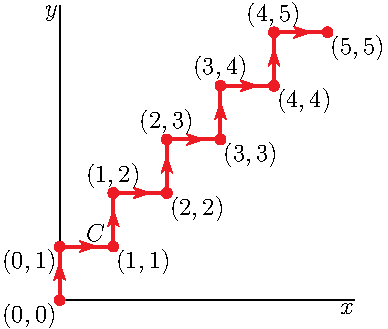
\includegraphics{OE06D_2.pdf}\qquad
       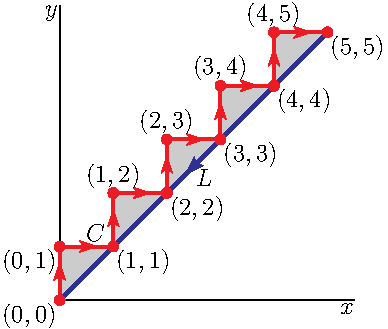
\includegraphics{OE06D_2b.pdf}
\end{center}
The curve $C$ is not closed, and so is not the boundary of a surface,
so we cannot apply Stokes' theorem directly. But we can easily
come up with a surface whose boundary contains $C$. Let $R$ be the shaded
region in the figure on the right above. The boundary $\partial R$ 
of $R$ consists of two parts --- $C$ and the line segment $L$.
The normal of $R$ for $-\hk$ (since $\partial R$ is oriented clockwise).
So Stokes' theorem gives
\begin{align*}
\int_C \vF \cdot\dee{\vr} + \int_L \vF \cdot\dee{\vr}
= \dblInt_R  \vnabla\times\vF \cdot(-\hk)\ \dee{S}
= \dblInt_R  (\hk) \cdot(-\hk)\ \dee{S}
= -\text{Area}(R)
\end{align*}
$R$ is the union of $5$ triangles, each of height $1$ and base $1$.
So
\begin{equation*}
\text{Area}(R) = 5\times \frac{1}{2}\times 1\times 1
=\frac{5}{2}
\end{equation*}
If we denote by $-L$ the line segment from $(0,0)$ to $(5,5)$,
we can parametrize $-L$ by $\vr(t) = t(5,5)$, $0\le t\le 1$ and
\begin{align*}
\int_{-L} \vF \cdot\dee{\vr}
&=\int_0^1 \overbrace{\big(5t\,\hi + (10t-10)\,\hj\big)}^{\vF(\vr(t))}
              \cdot\overbrace{(5\,\hi+5\,\hj)}^{\vr'(t)}\ \dee{t}
=\int_0^1 5\big(15t-10\big) \dee{t}
=25\left(\frac{3}{2}-2\right) \\
&=-\frac{25}{2}
\end{align*}
All together
\begin{align*}
\int_C \vF \cdot\dee{\vr} 
= -\text{Area}(R) - \int_L \vF \cdot\dee{\vr} 
= -\text{Area}(R) + \int_{-L} \vF \cdot\dee{\vr} 
=-\frac{5}{2}-\frac{25}{2}
=-15
\end{align*}
\end{solution}

%%%%%%%%%%%%%%%%%%%%%%%%%%%
\begin{question}[M317 2005A] %5
Let $\vF = \big(\sin x^2\,,\,xz\,,\,z^2\big)$.
Evaluate $\oint_C\vF\cdot\dee{\vr}$ around the curve $C$ of
intersection of the cylinder $x^2+y^2=4$ with the surface $z=x^2$, traversed
counter clockwise as viewed from high on the $z$-axis.
\end{question}

\begin{hint}
Direct evaluation looks hard.  
\end{hint}

\begin{answer} 
$12\pi$
\end{answer}


\begin{solution}
If we parametrize the curve as 
\begin{equation*}
x = 2\cos\theta\qquad 
y = 2\sin\theta\qquad
z= x^2 = 4\cos^2\theta\qquad
0\le\theta\le 2\pi
\end{equation*}
then the term $\sin x(\theta)^2\ x'(\theta)$ in the integral will be
$\sin\big(4\cos^2\theta\big)\ (-2\sin\theta)$. That looks hard to integrate.
So let's try Stokes' theorem.
The curl of $\vF$ is
\begin{align*}
\vnabla\times\vF
&=\det\left[\begin{matrix}
\hi &\hj &\hk \\
\tfrac{\partial\hfill}{\partial x} & \tfrac{\partial\hfill}{\partial y} & 
                \tfrac{\partial\hfill}{\partial z} \\
\sin x^2 & xz & z^2
\end{matrix}
\right]
=-x\,\hi +z\,\hk
\end{align*}
The curve $C$ is the boundary of the surface
\begin{equation*}
S = \Set{(x,y,z)}{x^2+y^2\le 4,\ z=x^2}
\end{equation*}
with upward pointing normal.
For the surface $z=f(x,y) = x^2$,
(\eref{CLP317}{eq:SUdSgraph}) in the CLP-4 text gives
\begin{align*}
\hn\, \dee{S} & = \pm\big[-f_x(x,y)\,\hi - f_y(x,y)\,\hj + \hk\big]\ 
          \dee{x}\dee{y}  \\
             & = \pm \big[-2x\,\hi+\hk\big]\,\dee{x}\dee{y}
\end{align*}
Since we want the upward pointing normal
\begin{align*}
\hn\, \dee{S} & = \big[-2x\,\hi+\hk\big]\,\dee{x}\dee{y}
\end{align*}
So by Stokes' theorem (Theorem \eref{CLP317}{thm:Stokes} in the CLP-4 text) 
\begin{align*}
\oint_C\vF\cdot\dee{\vr}
&=\dblInt_S \vnabla\times\vF \cdot \hn\,\dee{S}
=\dblInt_{x^2+y^2\le 4} \big(-x\,\hi + \overbrace{x^2}^{z}\hk\big)\cdot
\big[-2x\,\hi+\hk\big]\,\dee{x}\dee{y} \\
&=3\dblInt_{x^2+y^2\le 4} x^2\,\dee{x}\dee{y}
\end{align*}
Switching to polar coordinates
\begin{align*}
\oint_C\vF\cdot\dee{\vr}
&=3\int_0^2\dee{r}\,r\int_0^{2\pi}\dee{\theta}\ r^2\cos^2\theta \\
&=3\left[\int_0^2 r^3\,\dee{r}\right]
           \left[\int_0^{2\pi}\cos^2\theta\ \dee{\theta}\right] \\
&= 3\ \frac{2^4}{4} 
       \left[\int_0^{2\pi}\frac{\cos(2\theta)+1}{2}\ \dee{\theta}\right] \\
&= 12\pi
\end{align*}
For an efficient, sneaky, way to evaluate 
$\int_0^{2\pi} \cos^2 t\ \dee{t}$ see Example
\eref{CLP317}{eg:workIntegalB} in the CLP-4 text.

\end{solution}

%%%%%%%%%%%%%%%%%%%%%%%%%%%
\begin{question}[M317 2005A] %6
Explain how one deduces the differential form
\begin{equation*}
\vnabla\times\vE = -\frac{1}{c}\frac{\partial\vH}{\partial t}
\end{equation*}
of Faraday's law from its integral form
\begin{equation*}
\oint_C\vE\cdot\dee{\vr} = 
  -\frac{1}{c}\ \diff{\hfill}{t}\dblInt_S\vH\cdot\hn\,\dee{S}
\end{equation*}
\end{question}

\begin{hint} 
Rewrite $\oint_C\vE\cdot\dee{\vr}$ as a surface integral.
\end{hint}

\begin{answer} 
Rewrite $\oint_C\vE\cdot\dee{\vr}$ as a surface integral.  For the details,
see the solution.
\end{answer}


\begin{solution}
By Stokes' Theorem,
\begin{equation*}
\oint_C\vE\cdot \dee{\vr}=\dblInt_S(\vnabla\times\vE)\cdot \hn\,\dee{S}
\end{equation*}
so Faraday's law becomes 
\begin{equation*}
\dblInt_S\Big(\vnabla\times\vE
+\frac{1}{c}\frac{\partial\vH}{\partial t}\Big)\cdot\hn\,\dee{S}=0
\end{equation*}
This is true for all surfaces $S$. So the integrand, assuming that it is
continuous,  must be zero. 

To see this, let 
$\vG=\Big(\vnabla\times\vE+\frac{1}{c}\frac{\partial\vH}{\partial t}\Big)$.
Suppose that $\vG(\vx_0)\ne 0$. Pick a unit vector $\hn$ in the direction
of $\vG(\vx_0)$. Let $S$ be a very small flat disk centered on $\vx_0$
with normal $\hn$ (the vector we picked). Then $\vG(\vx_0)\cdot\hn>0$
and, by continuity, $\vG(\vx)\cdot\hn>0$ for all $\vx$ on $S$, if we have
picked $S$ small enough.
 Then $\dblInt_S\Big(\vnabla\times\vE
    +\frac{1}{c}\frac{\partial\vH}{\partial t}\Big)\cdot \hn\,\dee{S}>0$, which is a contradiction.
So $\vG=\vZero$ everywhere and we conclude that
\begin{equation*}
\vnabla\times\vE+\frac{1}{c}\frac{\partial\vH}{\partial t}=0
\end{equation*}
\end{solution}

%%%%%%%%%%%%%%%%%%%%%%%%%%%
\begin{question}[M317 2004A] %7
Let $C$ be the curve given by the parametric equations:
\begin{equation*}
x=\cos t,\ 
y=\sqrt{2}\sin t,\ 
z=\cos t,\ 
0\le t\le 2\pi
\end{equation*}
and let
\begin{equation*}
\vF=z\,\hi+x\,\hj+y^3z^3\,\hk
\end{equation*}
Use Stokes' theorem to evaluate 
\begin{equation*}
\oint_C \vF\cdot \dee{\vr}
\end{equation*}
\end{question}

\begin{hint} 
What is $x(t)^2+y(t)^2+z(t)^2=2$? How is $x(t)$
relatex to $z(t)$?
\end{hint}

\begin{answer} 
$\sqrt{2}\pi$
\end{answer}

\begin{solution} 
The curl of the specified vector field is
\begin{align*}
\nabla\times\vF
&=\nabla\times\big(z\,\hi+x\,\hj+y^3z^3\,\hk\big) \\
&= \det\left[\begin{matrix}
\hi & \hj & \hk \\
\tfrac{\partial\hfill}{\partial x} & \tfrac{\partial\hfill}{\partial y} & 
                \tfrac{\partial\hfill}{\partial z} \\
z & x & y^3z^3
\end{matrix}\right] \\
&=3y^2z^3\,\hi+\hj+\hk
\end{align*}
For every $t$, we have $x(t)=z(t)$ and $x(t)^2+y(t)^2+z(t)^2=2$.
So the specified curve is the intersection of the plane $x=z$ and the sphere
$x^2+y^2+z^2=2$. This curve is the boundary of the circular disk 
\begin{equation*}
D = \Set{(x,y,z)}{x=z,\ x^2+y^2+z^2\le 2}
\end{equation*}
The curve is oriented so that 
$\big(x(t),y(t)\big)=\big(\cos t,\sqrt{2}\sin t\big)$
runs in the standard (counterclockwise) direction. So the unit normal
to $D$ used in Stokes' theorem has positive $\hk$ component. Since the
plane $x-z=0$ has unit normal $\pm\frac{1}{\sqrt{2}}(1,0,-1)$, the unit
normal used in Stokes' theorem is $\hn=\frac{1}{\sqrt{2}}(-1,0,1)$. By Stokes'
theorem
\begin{align*}
\oint_C \vF\cdot \dee{\vr}
&=\dblInt_D\nabla\times\vF\cdot\hn\ \dee{S}
=\frac{1}{\sqrt{2}}\dblInt_D(3y^2z^3,1,1)\cdot(-1,0,1)\ \dee{S} \\
&=\frac{1}{\sqrt{2}}\dblInt_D(1-3y^2z^3)\ \dee{S}
\end{align*}
The disk $D$ is invariant under the reflection $(x,y,z)\rightarrow(-x,y,-z)$.
Since $y^2z^3$ is odd under this reflection, $\dblInt_D y^2z^3\ \dee{s}=0$
and
\begin{equation*}
\oint \vF\cdot \dee{\vr}
=\frac{1}{\sqrt{2}}\dblInt_D \ \dee{S}
=\frac{1}{\sqrt{2}}{\rm Area}(D)
\end{equation*}
Because the centre of the ball $x^2+y^2+z^2\le 2$ (namely $(0,0,0)$)
is contained in the plane $x=z$, the radius of the disk $D$ is the same
as the radius of the sphere $x^2+y^2+z^2=2$. So $D$ has radius $\sqrt{2}$ and
\begin{equation*}
\oint \vF\cdot \dee{\vr}
=\frac{1}{\sqrt{2}}{\rm Area}(D)
=\frac{1}{\sqrt{2}}\pi{\big(\,\sqrt{2}\,\big)}^2
=\sqrt{2}\pi
\end{equation*}
\end{solution}

%%%%%%%%%%%%%%%%%%%%%%%%%%%
\begin{question}[M317 2002A] %6
Use Stokes' theorem to evaluate 
$$
\oint_C z\,\dee{x}+x\,\dee{y}-y\,\dee{z}
$$
where $C$ is the  closed curve which is the intersection of the plane $x+y+z=1$
with the sphere $x^2+y^2+z^2=1$. Assume that $C$ is oriented  clockwise
as viewed from the origin.
\end{question}

\begin{hint} 
The intersection of the plane $x+y+z=1$ with the sphere $x^2+y^2+z^2=1$
is a circle. Use symmetry to guess the centre of the circle.
\end{hint}

\begin{answer} 
$\frac{2\pi}{3\sqrt{3}}$
\end{answer}

\begin{solution} 
The curl of the vector field $\vF=z\,\hi+x\,\hj-y\,\hk$ is
$$
\vnabla\times\vF=-\hi+\hj+\hk
$$
The unit normal to the plane $x+y+z=1$, with positive $\hk$ component as
required by Stokes' theorem in this case, is $\hn=\frac{1}{\sqrt{3}}(1,1,1)$.
If we denote by $D$ the circular disk $x+y+z=1$, $x^2+y^2+z^2\le 1$, then 
Stokes' theorem (Theorem \eref{CLP317}{thm:Stokes} in the CLP-4 text) says
\begin{align*}
\oint_C z\,\dee{x}+x\,\dee{y}-y\,\dee{z}=\oint_C \vF\cdot \dee{\vr}
&=\dblInt_D\vnabla\times\vF\cdot\hn\,\dee{S}
=\dblInt_D(-1,1,1)\cdot\frac{1}{\sqrt{3}}(1,1,1)\,\dee{S} \\
&=\frac{1}{\sqrt{3}}{\rm Area}(D)
\end{align*}
A reasonable guess for the centre of the disk is $\frac{1}{3}(1,1,1)$. 
(This guess is just based on symmetry.) To check
this we just need to observe that it is indeed on the plane $x+y+z=1$
and that the distance from  $\frac{1}{3}(1,1,1)$ to any point $(x,y,z)$
obeying $x+y+z=1$ and $x^2+y^2+z^2=1$, namely
\begin{align*}
\sqrt{{\Big(x-\frac{1}{3}\Big)}^2+{\Big(y-\frac{1}{3}\Big)}^2
+{\Big(z-\frac{1}{3}\Big)}^2}
&=\sqrt{x^2+y^2+z^2-\frac{2}{3}(x+y+z)+\frac{3}{9}}
=\sqrt{1-\frac{2}{3}+\frac{1}{3}}\\
&=\sqrt{\frac{2}{3}}
\end{align*}
is the same. This also tells us that $D$ has radius 
$\sqrt{\frac{2}{3}}$ and hence area $\frac{2}{3}\pi$. So the specified
line integral is $\frac{2\pi}{3\sqrt{3}}$.
\end{solution}


%%%%%%%%%%%%%%%%%%%%%%%%%%%
\begin{question}[M317 2018A] %7
Let $S$ be the part of the half cone 
\begin{equation*}
z=\sqrt{x^2+y^2},\quad  y\ge 0,
\end{equation*}
that lies below the plane $z=1$.
\begin{enumerate}[(a)]
\item
Find a parametrization for $S$.
\item
Calculate the flux of the velocity field
\begin{equation*}
\vv=x\,\hi + y\, \hj -2 z\,\hk
\end{equation*}
downward through $S$.

\item
A vector field $\vF$ has curl $\vnabla\times \vF= x\, \hi + y\, \hj -2 z\,\hk$. 
On the $xz$-plane, the vector field $\vF$ is constant with $\vF(x,0,z)=\hj$. Given this information, calculate
\begin{equation*}
\int_\cC \vF\cdot \dee{\vr},
\end{equation*}
where $\cC$ is the half circle
\begin{equation*}
x^2+y^2=1,\ z=1,\ y\ge 0
\end{equation*}
oriented from $(-1,0,1)$ to $(1,0,1)$.
\end{enumerate}
\end{question}

\begin{hint} 
Sketch $S$.
\end{hint}

\begin{answer} 
(a) One possible parametrization is 
$\vr(r, \theta) = r\cos \theta\, \hi +r\sin \theta\, \hj + r\,\hk$
with $0\le r\le 1$, $0\le \theta \le \pi$.

(b) $\pi$\qquad
\end{answer}

\begin{solution}  (a)
We parametrize $S$ in cylindrical coordinates:
\begin{equation*}
\vr(r, \theta) = r\cos \theta\, \hi +r\sin \theta\, \hj + r\,\hk
             \qquad \text{with $0\le r\le 1$, $0\le \theta \le \pi$}
\end{equation*}


(b) 
We compute
\begin{align*}
\frac{\partial \vr}{\partial r}
    &= \cos \theta \,\hi +\sin \theta \,\hj +\,\hk \\
\frac{\partial \vr}{\partial \theta} 
    &= -r \sin \theta \,\hi + r\cos \theta \,\hj \\
\hn\, \dee{S} &= \pm \frac{\partial \vr}{\partial r}\times 
                     \frac{\partial \vr}{\partial \theta} 
                   \ \dee{r}  \dee{\theta}
         = \pm \big(-r\cos \theta \,\hi - r \sin \theta \,\hj + r \,\hk\big)\,
                   \dee{r} \dee{\theta}
\end{align*}
To calculate the downward flux, we use the minus sign. We find
\begin{align*}
\dblInt_S \vv \cdot \hn\, \dee{S} 
& = \int_0^\pi \dee{\theta} \int_0^1 \dee{r}\  (r \cos \theta, r\sin \theta, -2r)\cdot 
                   (r\cos \theta, r\sin \theta, -r) \\
&= \int_0^\pi \dee{\theta} \int_0^1 \dee{r}\  3 r^2 
  = \pi r^3\Big|_{r=0}^1 = \pi
\end{align*}

(c) \emph{Solution 1}:\ \ \ 
Let $\cP$ be the path along line segments from $(1,0,1)$ to $(0,0,0)$ 
and from $(0,0,0)$ to $(-1,0,1)$. Here is a sketch. $\cP$ is
in blue.

\begin{center}
     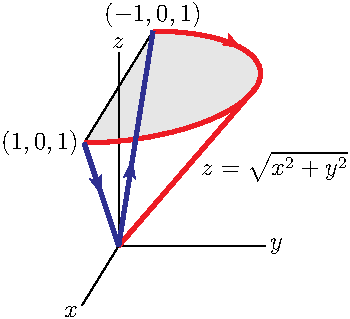
\includegraphics{halfCone.pdf}
\end{center}


Then
\begin{equation*}
\int_\cC \vF \cdot \dee{\vr} + \int_\cP \vF \cdot \dee{\vr} 
= \dblInt_S \vnabla \times \vF \cdot \hn\, \dee{S}
\end{equation*}
by Stokes' Theorem. Along $\cP$, the vector field $\vF$ is orthogonal 
to the curve so that $\int_\cP \vF\cdot \dee{\vr}=0$. Note that 
$\nabla\times \vF$ is the vector field $\vv$ from part (b). 
Thus
\begin{equation*}
\int_\cC \vF\cdot \dee{\vr} = \dblInt_S \vv \cdot \hn\, \dee{S} = \pi
\end{equation*}

(c) \emph{Solution 2:}\ \ \ 
Let $\cL$ be the  line segment from $(1,0,1)$ to $(-1,0,1)$ and
let 
\begin{align*}
\cR=\set{(x,y,z)}{x^2+y^2\le1, y\ge 0, z=1}
\end{align*}
Here is a sketch. $\cL$ is in blue and $\cR$ is shaded.

\begin{center}
     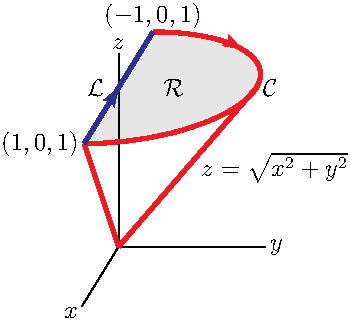
\includegraphics{halfConeB.pdf}
\end{center}

Then
\begin{equation*}
\int_\cC \vF \cdot \dee{\vr} + \int_\cL \vF \cdot \dee{\vr} 
= \dblInt_{\cR} \vnabla \times \vF \cdot (-\hk)\, \dee{S}
\end{equation*}
by Stokes' Theorem. Along $\cL$, the vector field $\vF=\hj$ is orthogonal 
to the curve (which has direction $-\hi$ so that $\int_\cL \vF\cdot \dee{\vr}=0$. Note that 
$\nabla\times \vF$ is the vector field $\vv$ from part (b). 
Thus
\begin{equation*}
\int_\cC \vF\cdot \dee{\vr} = -\dblInt_\cR \vv \cdot \hk\, \dee{S}
= \dblInt_\cR 2z \, \dee{S} 
= 2\dblInt_\cR \, \dee{S} 
=2\,\text{Area}(\cR)
= \pi
\end{equation*}

\end{solution}

%%%%%%%%%%%%%%%%%%%%%%%%%%%%%%%
\begin{question}
Consider $\dblInt_S(\vnabla\times\vF)\cdot\hn\,dS$ where $S$
is the portion of the sphere $x^2+y^2+z^2=1$ that obeys $x+y+z\ge 1$, $\hn$
is the upward pointing normal to the sphere and
 $\vF=(y-z)\hi+(z-x)\hj+(x-y)\hk$. Find another
surface $S'$ with the property that $\dblInt_S(\vnabla\times\vF)\cdot\hn\,\dee{S}
=\dblInt_{S'}(\vnabla\times\vF)\cdot\hn\,\dee{S}$ and evaluate
$\dblInt_{S'}(\vnabla\times\vF)\cdot\hn\,\dee{S}$.
\end{question}

\begin{hint} 
You can avoid evaluating any integral
by identifying $S'$ as a simple geometric figure.
\end{hint}

\begin{answer} 
$-\frac{4}{\sqrt{3}}\pi$
\end{answer}

\begin{solution} 
Let $S'$ be the portion of $x+y+z=1$ that is inside the sphere
$x^2+y^2+z^2=1$. Then $\partial S=\partial S'$, so, by  Stokes' theorem,
(with $\hn$ always the upward pointing normal)
\begin{equation*}
\dblInt_{S'}(\vnabla\times\vF)\cdot\hn\,\dee{S}
=\oint_{\partial S'}\vF\cdot \dee{\vr}
=\oint_{\partial S}\vF\cdot \dee{\vr}
=\dblInt_{S}(\vnabla\times\vF)\cdot\hn\,\dee{S}
\end{equation*}
As
\begin{align*}
\vnabla\times\vF=\det\left[\begin{matrix}\hi & \hj & \hk \\[0.05in]
                  \pdiff{}{x} &
                  \pdiff{}{y} &
                  \pdiff{}{z} \\[0.05in]
                  y-z & z-x & x-y \end{matrix}\right] 
=-2(\hi+\hj+\hk)
\end{align*}
and, on $S'$,  
$\hn=\frac{1}{\sqrt{3}}(\hi+\hj+\hk)$
\begin{equation*}
\dblInt_{S'}(\vnabla\times\vF)\cdot\hn\,\dee{S}
=\dblInt_{S'}\big(-2\sqrt{3}\big)\,\dee{S}
=-2\sqrt{3}\times{\rm Area}(S')
\end{equation*}
$S'$ is the intersection of a plane with a sphere and so is a circular disk. It's center $(x_c,y_c,z_c)$ has to obey 
$x_c+y_c+z_c=1$. By symmetry, $x_c=y_c=z_c$, so $x_c=y_c=z_c=\frac{1}{3}$.
Any point, $(x,y,z)$, which satisfies both $x+y+z=1$ and $x^2+y^2+z^2=1$,
obeys
\begin{align*}
\left(x-\frac{1}{3}\right)^2+\left(y-\frac{1}{3}\right)^2
+\left(z-\frac{1}{3}\right)^2
=x^2+y^2+z^2-\frac{2}{3}(x+y+z)+3\frac{1}{9}
=1-\frac{2}{3} +\frac{1}{3}=\frac{2}{3}
\end{align*}
That is, any point on the boundary of $S'$ is a distance $\sqrt{\frac{2}{3}}$
from $\big(\frac{1}{3}\,,\,\frac{1}{3}\,,\,\frac{1}{3}\big)$.  
So the radius of $S'$ is $\sqrt{\frac{2}{3}}$,
the area of $S'$ is $\frac{2}{3}\pi$ and 
\begin{equation*}
\dblInt_{S'}(\vnabla\times\vF)\cdot\hn\,\dee{S}
=-2\sqrt{3}\times{\rm Area}(S')
=-\frac{4}{\sqrt{3}}\pi
\end{equation*}

\end{solution}






